%%%%%%%%%%%%%%%%%%%%%%%%%%%%%%%%%%%%%
%% Projeto Final - Arquivo principal
%% UNIVERSIDADE C�NDIDO MENDES - Bacharel em Ci�ncias da Computa��o
%% Projeto final: M�dulo de Mapeamento do Toolkit H�rus.
%% J�natas Oliveria Lopes Soares / Maycon Barreto Lopes / Wallace Gomes de Souza
%% Orientador: Prof. D. �talo Matias
%% Campos dos Goytacazes - RJ
%% 2009
%%%%%%%%%%%%%%%%%%%%%%%%%%%%%%%%%%%%%%

\documentclass[a4paper,12pt]{report}
%Configura��o geral
\usepackage{a4wide}
\usepackage[brazil,english]{babel}
\usepackage{graphicx}
\usepackage{amsmath}
\usepackage{epsfig}
\usepackage[latin1]{inputenc}
\usepackage{doublespace}
\usepackage{fancyheadings}
\usepackage{longtable}
\usepackage{dropping}
\usepackage{url}
\usepackage{subfigure}
\usepackage{abntcite}
\usepackage{textcomp}
\usepackage{algorithmic}
\def\citeopen{[}
\def\citeclose{]}

\newcommand{\figr}[1]{Figura~\ref{#1}}
\newcommand{\eqt}[1]{Eq.~(\ref{#1})}
\newcommand{\eqts}[2]{Eq.~(\ref{#1})~e~(\ref{#2})}
\newcommand{\eqtss}[3]{Eq.~(\ref{#1})~,~(\ref{#2})~e~(\ref{#3})}
\newcommand{\tab}[1]{Tabela~\ref{#1}}

%Comandos para se definir cabe�alhos nas p�ginas da disserta��o
\pagestyle{fancyplain}
\lhead[\fancyplain{}{\thepage}]{\fancyplain{}{\small\leftmark}}
\rhead[\fancyplain{}{\small\rightmark}]{\fancyplain{}{\thepage}}
\cfoot{\fancyplain{\thepage}{}}

%Configura��o para numera��o de subsubse��es
\setcounter{secnumdepth}{3}

%Instancia do contador que ser� usado como refer�ncia na monografia
\newcounter{mypage}

% Frases de efeito no in�cio de cada cap�tulo
\newcommand{\epigraph}[2]{%
  \vspace{1ex}%
  {\footnotesize%
   \begin{spacing}{1}
    \begin{flushright}%
      \begin{minipage}{.6\textwidth}%
        #1\\
      \end{minipage}\\
      \textit{#2}%
    \end{flushright}
    \end{spacing}}%
  \vspace{1ex}}

\DeclareGraphicsExtensions{.jpg, .pdf, .mps, .png}

\begin{document}
 \stepcounter{mypage}

%--------------------------------
%  PRIMEIRAS P�GINAS
%--------------------------------
%Include da capa
%%%%%%%%%%%%%%%%%%%%%%%%%%%%%%%%%%%%%
%% Projeto Final - Arquivo principal
%% UNIVERSIDADE C�NDIDO MENDES - Bacharel em Ci�ncias da Computa��o
%% Projeto final: M�dulo de Mapeamento do Toolkit H�rus.
%% J�natas Oliveria Lopes Soares / Maycon Barreto Lopes / Wallace Gomes de Souza
%% Orientador: Prof. D. �talo Matias
%% Campos dos Goytacazes - RJ
%% 2009
%%%%%%%%%%%%%%%%%%%%%%%%%%%%%%%%%%%%%%


\thispagestyle{empty}

\begin{spacing}{1.0}

\begin{center}
\begin{large}
UNIVERSIDADE C�NDIDO MENDES
\end{large}
\end{center}

\vspace {2 cm}
\begin{center}
\begin{large}
\uppercase{
J�natas Oliveria Lopes Soares \par Maycon Barreto Lopes \par Wallace Gomes de Souza
}
\end{large}
\end{center}
\vspace {4 cm}
\begin{spacing}{1.5}
\begin{center}
\begin{huge}
{\bf \uppercase{
M�dulo de Mapeamento do ToolKit H�rus}
}
\end{huge}

\end{center}
\end{spacing}

\vspace {8 cm}

\begin{center}

\begin{large}
Campos dos Goytacazes - RJ \\[0.2 cm]
2009
\end{large}
\end{center}

\end{spacing}
\newpage




\stepcounter{mypage}
%Include da folha de rosto
%%%%%%%%%%%%%%%%%%%%%%%%%%%%%%%%%%%%%
%%   Folha de rosto
%%%%%%%%%%%%%%%%%%%%%%%%%%%%%%%%%%%%%


\thispagestyle{empty}

\begin{spacing}{1.0}

\begin{center}
\begin{large}
\uppercase{
J�natas Oliveira Lopes Soares \par Maycon Barreto Lopes \par Wallace Gomes de Souza} \\[0.2 cm]
\end{large}
\end{center}

\vspace {6 cm}

\begin{spacing}{1.5}
\begin{center}
\begin{huge}
{\bf \uppercase{M�dulo de Mapeamento do ToolKit H�rus}}
\end{huge}
\end{center}
\end{spacing}

\vspace {2 cm}

\begin{flushright}
\begin{minipage}[t]{8.5 cm}
Monografia apresentada � Universidade C�ndido Mendes como requisito obrigat�rio para a obten��o do grau de Bacharel em Cin�ncias da Computa��o.
\end{minipage}
\end{flushright}

\vspace {1.5 cm}

\begin{center}
\begin{large}
ORIENTADOR: Prof. D.Sc. �talo Matias\\[0.2 cm]
\end{large}
\end{center}

\begin{center}
\begin{large}
CO-ORIENTADOR: Prof. D.Sc. Dalessandro Soares \\[0.2 cm]
\end{large}
\end{center}

\vspace {1.5 cm}

\begin{center}
\begin{large}
Campos dos Goytacazes-RJ\\[0.2 cm]
2009
\end{large}
\end{center}

\end{spacing}
\newpage


\stepcounter{mypage}
%Include da folha de aprova��es
%%%%%%%%%%%%%%%%%%%%%%%%%%%%%%%%%%%%%
%%   Folha de aprova��o
%%%%%%%%%%%%%%%%%%%%%%%%%%%%%%%%%%%%%


\thispagestyle{empty}

\begin{spacing}{1.0}

\begin{center}
\begin{large}
\uppercase{
J�natas Oliveria Lopes Soares \par Maycon Barreto Lopes \par Wallace Gomes de Souza
}
\end{large}
\end{center}

\vspace {1.0 cm}

\begin{center}
\begin{large}
{\bf \uppercase{
M�dulo de Mapeamento do ToolKit H�rus}
} \\[0.2 cm]
\end{large}
\end{center}

\vspace {1.0 cm}

\begin{flushright}
\begin{minipage}[t]{8.5 cm}
Monografia apresentada � Universidade C�ndido Mendes como requisito obrigat�rio para a obten��o do grau de Bacharel em Cin�ncias da Computa��o.
\end{minipage}
\end{flushright}

\vspace {1.5 cm}

\begin{center}
\begin{large}
Aprovada em \_\_\_\_ de \_\_\_\_\_\_\_\_\_\_\_\_ de 2009. \\[0.2 cm]
\end{large}
\end{center}

\vspace {1.5 cm}

\begin{center}
\begin{large}
BANCA EXAMINADORA \\[0.2 cm]
\end{large}
\end{center}

\vspace {1.5 cm}

\begin{center}
\line(1,0){300}\\ 
Prof. D.Sc. �talo Matias - Orientador \\
Doutor pela UFRJ
\end{center}

\vspace {1.0 cm}

\begin{center}
\line(1,0){300}\\ 
Prof. D.Sc. Dalessandro Soares\\
Doutor pela PUC-Rio
\end{center}

\vspace {1.0 cm}

\begin{center}
\line(1,0){300}\\ 
Prof. BLABLABLA\\
Univeridade de Londres
\end{center}


\end{spacing}
\newpage

\stepcounter{mypage}
%Include da dedicat�ria
%%%%%%%%%%%%%%%%%%%%%%%%%%%%%%%%%%%%%
%%  DEDICAT�RIA
%%%%%%%%%%%%%%%%%%%%%%%%%%%%%%%%%%%%%


\thispagestyle{empty}

\

\vfill

\begin{flushright}
\hfill \textit{Dedico este trabalho a minha m�e, irm� e namorada. \\
 J�natas}
\vspace*{1cm}

\textit{
Dedico este trabalho a meus pais.
\\ Maycon}

\vspace*{1cm}

\textit{
Dedico este trabalho a meus pais.
\\ Wallace}

\end{flushright}

\vspace*{1cm}

\clearpage

\stepcounter{mypage}
%Include dos agradecimentos
%%%%%%%%%%%%%%%%%%%%%%%%%%%%%%%%%%%%%
%%  AGRADECIMENTOS
%%%%%%%%%%%%%%%%%%%%%%%%%%%%%%%%%%%%%


\chapter*{Agradecimentos}
\thispagestyle{empty}
Agradecemos as nossas fam�lias e amigos, pela paci�ncia e apoio, que possibilitou calma e for�as para o desenvolvimento desse projeto, assim como durante todos os momentos dif�ceis ao longo de nossa gradua��o. Agradecemos aos orientadores Italo de Oliveira Matias e Dalessandro Soares Vianna pelo apoio e orienta��o para o desenvolvimento desse trabalho, assim como a Universidade Candido Mendes por propiciar um ambiente frut�fero a pesquisa e aprendizado.


\thispagestyle{empty} 


% Caso passe de p�gina adicionar essa linha para  que n�o seja reformatada
% inserir o restante do texto abaixo dela.
% \thispagestyle{empty} 


\stepcounter{mypage}


%-----------------------------------
% DOCUMENTA��O DO TRABALHO
%-----------------------------------
\renewcommand{\baselinestretch}{1.3}

%-----------------------------------
% NUMERA��O DE P�GINA EM ROMANO
%-----------------------------------
\pagenumbering{roman}
\setlength{\voffset}{0.0in}

%Atribui ao contador page (default do latex, que � usado por todo o documento)
%o valor do contador � mypage
\setcounter{page}{\value{mypage}}

%Espa�amento das p�ginas
\begin{spacing}{1.5}
%Include do resumo
%%%%%%%%%%%%%%%%%%%%%%%%%%%%%%%%%%%%%
%%   Resumo
%%%%%%%%%%%%%%%%%%%%%%%%%%%%%%%%%%%%%


\chapter*{Resumo}
Neste trabalho, ser�o apresentados os conceitos e algoritmos envolvidos na constru��o de um \textit{toolkit Open Source}, de nome Horus, utilizado para o desenvolvimento e controle de aplica��es que envolvam agentes inteligentes, com foco em dois problemas centrais. O primeiro problema refere-se � movimenta��o aut�noma de um agente inteligente em ambientes desconhecidos. O segundo problema refere-se �  vis�o computacional, onde o agente deve ser capaz de extrair informa��es do ambiente atrav�s da utiliza��o de c�meras virtuais ou reais. Al�m de algoritmos para movimenta��o aut�noma e vis�o computacional, o Horus tamb�m fornece abstra��es para cria��o e configura��o de agentes inteligentes com seus principais componentes e dispositivos. Embora o Horus tenha sido tamb�m desenvolvido com foco na movimenta��o aut�noma de agentes inteligentes, nesse trabalho ser� dado maior enfoque � parte de vis�o computacional e �s abstra��es para cria��o e configura��o de agentes inteligentes. Como forma de valida��o e prova de conceito das funcionalidades fornecidas pelo toolkit Horus, tamb�m foram desenvolvidas tr�s aplica��es: PyANPR, Teseu e Ariadnes. PyANPR � um sistema \textit{web} de reconhecimento autom�tico de placas de autom�veis. Teseu � um sistema que simula o mapeamento autom�tico de um ambiente desconhecido por um agente inteligente. Ariadnes � um sistema que simula a movimenta��o aut�noma de um agente inteligente em um ambiente desconhecido atrav�s de t�cnicas de vis�o computacional e mapeamento de ambientes. Neste trabalho, al�m da descri��o do Horus, tamb�m ser�o detalhadas a aplica��o PyANPR e os aspectos de vis�o computacional do simulador Ariadnes.



\vspace{0.5cm}

Palavras-chave: Vis�o Computacional, Mapeamento de Ambientes, Horus

\end{spacing}

\begin{spacing}{1.5}
%Include do abstract
%%%%%%%%%%%%%%%%%%%%%%%%%%%%%%%%%%%%%
%%   Abstract
%%%%%%%%%%%%%%%%%%%%%%%%%%%%%%%%%%%%%


\chapter*{Abstract}

This work was carried through with intention to compare and to evaluate four of the main techniques of limiarization and image segmentation, applied to the picture processing of wooden stack photos, as solution for the calculation of piling factors.  Between these techniques, we considered the segmentation based in the use of the Non Extensive Entropy, also known as Tsallis Entropy \cite{Tsallis_1988,Tsallis_1999,Tsallis_2001}, applied to this problem.  For this, we had been implemented each one of the tested techniques through a software that was developed.  Tests with photos of stacks manually piled up on the ground had been made; and the results of each technique had been compared with the manual measures  made in field.  The objective of this work is, through the results of the experiments, to verify which of the tested algorithms adjusts better to the automatic calculation of the piling factors, using image segmentation.

%This work was carried through with intention to compare and to evaluate four amongst the diverse techniques of limiarization and segmentation of images, applied to the picture processing of wooden stack photos, as solution for the calculation of piling factors.  Between these techniques, we considered  the segmentation carried through the use of the Not Extensive Entropy, also known as Tsallis Entropy \cite{Tsallis_1988}, applied to this problem.  For this, they had been implemented each one of the tested techniques through a small software that was developed.  Tests with photos of stacks manually on the ground had been carried through; and the results of each technique had been compared with the carried through manual measurements in field.  The objective of this work is, through the carried through experiments, to get for the process of segmentation of images, a precise result in the calculation of the piling factors and to suggest which of the tested algorithms adjusts better to the considered problem.

\vspace{0.5cm}
Keywords:  Piling factors, digital photos, Tsallis Entropy, Image Segmentation 

\end{spacing}

\selectlanguage{brazil}

%�ndices
\begin{spacing}{1.0}
%�ndice de cap�tulos
\tableofcontents
%�ndice de figuras
\listoffigures
%�ndice de tabelas
\listoftables
\end{spacing}

\clearpage

% Atribuindo ao nosso contador o valor do contador page
% e depois incremento...
\setcounter{mypage}{\value{page}}
\clearpage

\pagenumbering{arabic}

%Includes da monografia propriamente dita
\begin{spacing}{1.5}
\setcounter{page}{\value{mypage}} % Atribuindo o contador page novamente....
%%%%%%%%%%%%%%%%%%%%%%%%%%%%%%%%%%%%%
%%   Introdu��o
%%%%%%%%%%%%%%%%%%%%%%%%%%%%%%%%%%%%%


\chapter{Introdu��o}

Existem alguns tipos de ambiente que s�o in�spitos ao homem. Nesses casos � comum utilizar um rob� para explorar e atuar em tais locais. A movimenta��o desses rob�s pode ser autom�tica (agentes aut�nomos), semi-autom�tica (agentes semi-aut�nomos) ou manuais. Neste trabalho, ser�o apresentados os passos para a constru��o de um \textit{toolkit}, de nome Horus, utilizado para o desenvolvimento e controle de aplica��es que envolvam agentes inteligentes, com foco em dois problemas centrais. O primeiro problema refere-se a movimenta��o aut�noma de um agente inteligente em ambientes desconhecidos. O segundo problema refere-se �  vis�o computacional, onde o agente deve ser capaz de extrair informa��es do ambiente atrav�s da utiliza��o de c�meras virtuais ou reais.

Um Agente, por defini��o, � todo elemento ou entidade aut�noma que pode perceber seu ambiente, por algum meio cognitivo ou sensorial, e de agir sobre esse ambiente por interm�dio de atuadores. Pode-se citar como exemplos de agentes inteligentes, al�m de um rob� aut�nomo ou semi-aut�nomo, personagens de um jogo,
agentes de busca e recupera��o de informa��o, entre outros.

Para que um agente aut�nomo seja capaz de atuar em um ambiente desconhecido � necess�rio anteriormente explorar esse local. Essa explora��o pode ser feita atrav�s de um mapeamento desse ambiente. A forma como mapeia-se o ambiente internamente no sistema � determinante na sua precis�o e performance. As diferentes abordagens para controle de agentes m�veis aut�nomos interagem fortemente com a representa��o do ambiente. Uma proposta para mapeamento do ambiente, ainda n�o implementada no Horus, � construir um ambiente virtual 3D associado a um ambiente real no qual um rob� real est� explorando. Essa abordagem exige que o agente reconhe�a padr�es no ambiente explorado e represente-os no ambiente virtual. 

 Durante a explora��o do ambiente, o agente dever� ser capaz de estimar sua posi��o local para localizar-se globalmente e se recuperar de poss�veis erros de localiza��o. Um correto mapeamento do ambiente junto a aplica��o correta das leis da cinem�tica podem resolver tal problema. Uma proposta para a localiza��o de um agente no ambiente � a utiliza��o do m�todo Monte Carlo [5] ou do m�todo SLAM (\textit{Simultaneous Location and Mapping}) [6], [7]. O m�todo selecionado para ser implementado no \textit{toolkit} horus foi o SLAM.

 Um agente explora um ambiente atrav�s de sensores. O sensoriamento prov� ao rob� as informa��es necess�rias para a constru��o de uma representa��o do ambiente onde est� inserido e para uma intera��o com os elementos contidos nesse. Sistemas com uma variedade de sensores tendem a obter resultados mais precisos. A fus�o de dados de sensores, ou como � mais conhecida, fus�o de sensores, � o processo de combina��o de dados de m�ltiplos sensores para estimar ou predizer estados dos elementos da cena. Neste trabalho, foram utilizados lasers, c�meras e od�metro como sensores.

 Para simular a vis�o de um agente inteligente, s�o utilizadas c�meras virtuais. Na abordagem desse trabalho, a vis�o � a principal forma de percep��o do ambiente. A vis�o possibilita reconhecer padr�es e classificar obst�culos.
Existem diferentes tipos de obst�culos. Estes podem se classifcados como transpon�vel (aquele que n�o interrompe a trajet�ria), intranspon�vel (aquele que o exigir� recalcula a trajet�ria por outro caminho) e redutor (aquele que permite ao rob� seguir pela trajet�ria, por�m a uma velocidade mais lenta). Mesmo mediante a obst�culos transpon�veis e redutores, pode ser conveniente recalcular o caminho devido ao aumento do custo do percurso. Uma proposta para o desvio de trajet�ria � o modelo baseado em Campos Potenciais proposto por [8]. A classifica��o de um obst�culo ocorre mediante a algum m�todo de reconhecimento de padr�es, baseado em vis�o computacional.

O \textit{toolkit} Horus prop�e uma cole��o de classes e algoritmos voltados a resolu��o de problemas pertencentes as �reas de vis�o computacional e mapeamento autom�tico de ambientes. Nessa monografia, ser� dado foco � parte de vis�o computacional do Horus. De forma a validar a implementa��o do \textit{toolkit} e demonstrar a sua utilidade, foram desenvolvidas tr�s aplica��es distintas: Os simuladores Teseu e Ariadnes, e o ANPR Django. Neste trabalho, al�m do \textit{toolkit} Horus, ser�o, tamb�m, apresentados a parte de vis�o computacional utilizada no simulador Ariadnes e a aplica��o para reconhecimento autom�tico de placas de autom�veis ANPR Django.

%%%%%%%%%%%%%%%%%%%%%%%%%%%%%%%%%%%%%
%%  INTELIG�NCIA ARTIFICIAL
%%%%%%%%%%%%%%%%%%%%%%%%%%%%%%%%%%%%%


\chapter{Intelig�ncia Artificial}
\label{cap:inteligencia_artificial}
\section{Agentes Inteligentes}
Ol� voc� est� aqui. \cite{Christiam_2005}
\section{Teste de Turing}
\section{T�cnicas de IA}
\subsection{RNA}
\subsection{Algoritmos Gen�ticos}
\subsection{L�gica Fuzzy}

%%%%%%%%%%%%%%%%%%%%%%%%%%%%%%%%%%%%%
%%  Extra��o de Caracter�sticas
%%%%%%%%%%%%%%%%%%%%%%%%%%%%%%%%%%%%%


\chapter{Horus}
\label{cap:horus}
 Horus � um \textit{toolkit}, criado no presente trabalho, para desenvolvimento e controle de agentes inteligentes desenvolvido na linguagem de programa��o Python. Esse \textit{toolkit} foi constru�do com o objetivo de fornecer classes e algoritmos voltados a resolu��o de problemas de mapeamento autom�tico de ambientes e vis�o computacional.

	O \textit{toolkit} Horus fornece os m�dulos \textit{Core}, Mapeamento, Vis�o e Util. O m�dulo \textit{Core} apresenta as abstra��es que devem ser implementadas pelas aplica��es para construir um agente inteligente. O m�dulo Mapeamento fornece algoritmos de localiza��o, mapeamento e navega��o para um agente. O m�dulo Vis�o fornece os algoritmos de vis�o computacional necess�rios na etapa de reconhecimento de padr�es. Por �ltimo, o m�dulo Util fornece um conjunto de fun��es utilit�rias eque podem ser usadas tanto no \textit{toolkit} Horus quanto em qualquer outra aplica��o. Cada um desses m�dulos ser� explicado nas subse��es seguintes.

\section{\textit{Core}}

	O Horus pode ser utilizado tanto como uma biblioteca de algoritmos para processamento de imagens, vis�o computacional e mapeamento de ambientes, como atrav�s de extens�es das classes fornecidas pelo m�dulo \textit{core}. Essas classes, podem ser estendidas pelas aplica��es, s�o chamadas de abstra��es. A Figura \ref{fig:arquiteturaCore} mostra a arquitetura deste m�dulo.

\begin{figure}[!htb]
\centering
\begin{center}
    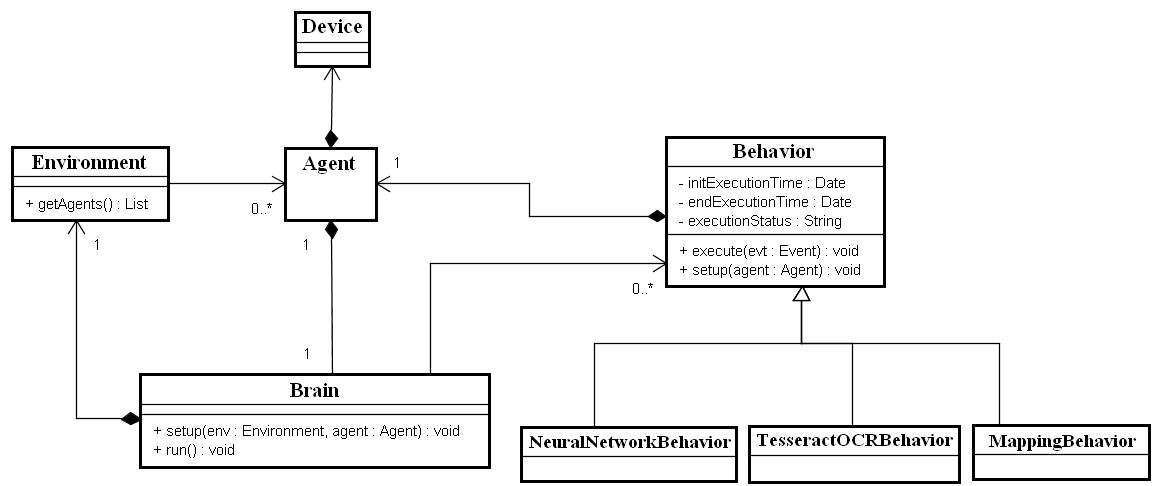
\includegraphics[scale=0.35, bb=0 0 1158 486]{imagens/core.PNG}
\end{center}
\caption{Arquitetura do m�dulo \textit{core}.}
\label{fig:arquiteturaCore}
\end{figure}

	A arquitetura acima apresenta classes que representam o ambiente (\textit{Environment}), o agente inteligente (\textit{Agent}), os dispositivos (\textit{Device}), o programa de agente (\textit{Brain}), eventos (\textit{Event}) e a hierarquia de comportamentos (\textit{Behavior}). Cada inst�ncia da classe \textit{Agent} representa um agente inteligente na aplica��o. Para que um agente inteligente possa ser utilizado por uma aplica��o, ela deve configur�-lo com inst�ncias de \textit{Device} e uma �nica inst�ncia da classe \textit{Brain}, respons�vel pela intelig�ncia do agente.

	O programa de agente, respons�vel pela intelig�ncia do agente, deve ser implementado em extens�es da classe \textit{Brain} (c�rebro). Uma aplica��o que deseja implementar um programa de agente para um agente em particular deve estender a classe \textit{Brain} e implementar o m�todo \textit{run()} dessa classe, como apresentado na Figura \ref{fig:arquiteturaBrain}. Esse m�todo � o \textit{loop} principal da execu��o do agente. No diagrama acima, nota-se que a classe \textit{Brain} pode estar relacionada a nenhum ou a muitos comportamentos. Essa � mais uma facilidade fornecida pelo m�dulo \textit{core} do Horus que tem o objetivo de organizar a implementa��o dos comportamentos separadamente da implementa��o da classe \textit{Brain}. Dessa forma, o programa de agente fica mais claro e simples de ser compreendido e mantido.

\begin{figure}[!htb]
\centering
\begin{center}
    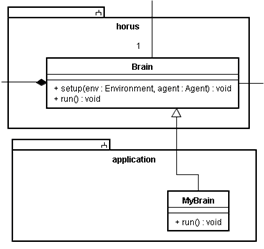
\includegraphics[scale=0.4, bb=0 0 561 544]{imagens/brainExtension.PNG}
\end{center}
\caption{Extens�o da classe \textit{Brain} do Horus por uma aplica��o.}
\label{fig:arquiteturaBrain}
\end{figure}

Os comportamentos (\textit{Behavior}) recebem eventos gerados pela aplica��o e fazem com que o agente execute uma determinada a��o com base no tipo de evento recebido. Como exemplo de eventos, pode-se citar a captura de uma cena, um obst�culo detectado, a leitura de um determinado dispositivo, etc. Um comportamento pode ser implementado diretamente como uma extens�o da classe \textit{Behavior} ou como uma extens�o de uma ou v�rias de suas subclasses. As subclasses da classe \textit{Behavior} (\textit{NeuralNetworkBehavior}, \textit{TesseractBehavior} e \textit{MappingBehavior}) fornecem facilidades para a utiliza��o de funcionalidades fornecidas pelo Horus. Logo, \textit{NeuralNetworkBehavior} fornece m�todos para a constru��o e treinamento de redes neurais na implementa��o de um comportamento. A classe \textit{TesseractBehavior} disponibiliza a funcionalidade de OCR da \textit{engine} Tesseract, presente no Horus. A classe \textit{MappingBehavior} disponibiliza m�todos para implementa��o de comportamentos de mapeamento de ambientes atrav�s da t�cnica SLAM. Dessa forma, uma aplica��o que necessite de um comportamento que envolva mapeamento de ambientes e redes neurais, por exemplo, deve criar uma classe que estenda tanto da classe \textit{MappingBehavior} como da classe \textit{NeuralNetworkBehavior}. A Figura \ref{fig:arquiteturaBehavior} mostra como ficaria o esquema desse comportamento, sendo representado pela classe \textit{MyBehavior}.

A classe \textit{Behavior} tamb�m possui atributos para armazenar informa��es sobre estado de execu��o de um comportamento. Essas informa��es s�o os hor�rios de in�cio e t�rmino da execu��o e o status de execu��o do comportamento. Essas informa��es s�o utilizadas para emiss�o de relat�rios de atua��o do agente.

\begin{figure}[!htb]
\centering
\begin{center}
    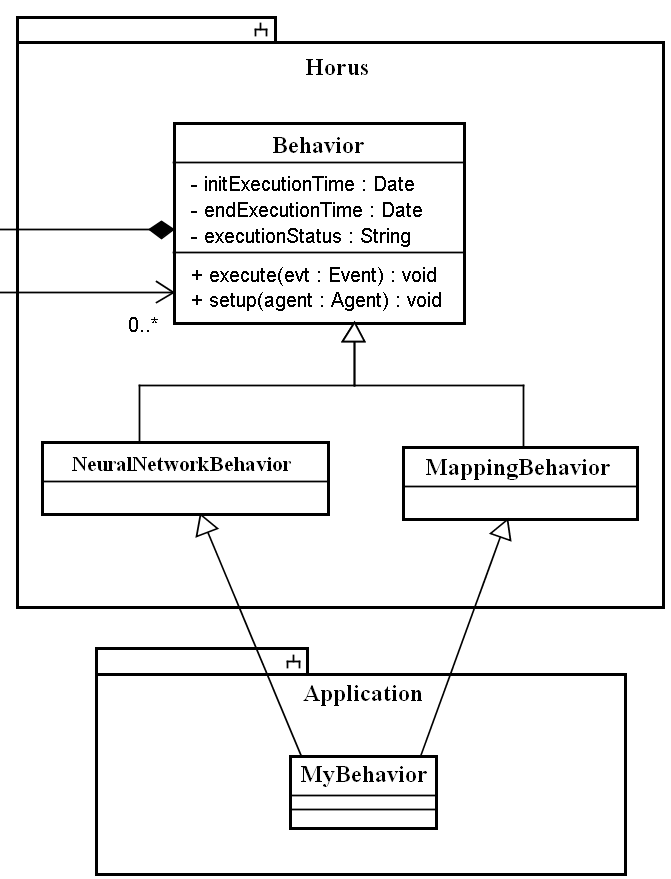
\includegraphics[scale=0.35, bb=0 0 671 879]{imagens/behaviorExtension.PNG}
\end{center}
\caption{Comportamento \textit{MyBehavior} que estende tanto de \textit{NeuralNetworkBehavior} quanto de \textit{MappingBehavior}.}
\label{fig:arquiteturaBehavior}
\end{figure}

Em certas aplica��es, um agente inteligente n�o necessariamente se encontra sozinho no ambiente. Ele pode interagir com outros agentes, como no caso de aplica��es que envolvam enxames de agentes. Para que um agente possa obter informa��es sobre outros agentes que se encontrem no ambiente, ou sobre o pr�prio ambiente, foi criada a classe \textit{Environment}, que representa o ambiente no qual o agente est� inserido. Dessa forma, o c�rebro do agente deve ser configurado tanto com uma inst�ncia da classe \textit{Agent}, como com uma inst�ncia da classe \textit{Environment} para operar.

Quando o c�rebro do agente � configurado com diversos comportamentos, � necess�rio definir a ordem de execu��o desses comportamentos. Em alguns casos, os comportamentos podem possuir condi��es de execu��o. Logo, o c�rebro � respons�vel por identificar as condi��es que cada comportamento necessita para ser executado e coloc�-lo como ativo quando a sua condi��o de execu��o for satisfeita. Contudo, h� casos em que dois ou mais comportamentos podem ter a sua condi��o de execu��o satisfeita. Nesses casos, � necess�rio definir prioridades de execu��o sobre os comportamentos ou execut�-los em paralelo. A ordem de execu��o dos comportamentos define a m�quina de estados de execu��o do agente inteligente. Sendo assim, a implementa��o do c�rebro como uma m�quina de estados se enquadra perfeitamente em aplica��es que exijam a intera��o entre diversos comportamentos.

\section{Processamento de Imagem}
\label{image:processing}

O termo processamento de imagens refere-se ao processamento de imagens de duas dimens�es por um computador digital [LIVRO FUNDAMENTALS OF DIGITAL IMAGE PROCESSING], normalmente � utilizado como um est�gio para novos processamentos de dados, tais como reconhecimento de padr�es e aprendizagem de m�quina. Esse tipo de processamento � utilizado em diversos tipos de aplica��es, entre elas, processamento de imagens m�dicas e de sat�lite, rob�tica, sensoriamento remoto, entre outras.

Para uma melhor compreens�o dos conceitos e algoritmos utilizados durante esse trabalho, � necess�rio uma breve introdu��o sobre algumas propriedades de uma imagem digital. Essas propriedades s�o:

\begin{itemize}

\item Conectividade: esse conceito determina se dois pixels est�o conectados entre si. Para isso, � necess�rio determinar se esses pixels s�o adjacentes, segundo algum crit�rio, e se os seus n�veis de cinza s�o, de alguma forma, similares. Definindo uma image bin�ria onde os pixels somente assumem valores 0 e 1, dois pixels vizinhos s� ser�o considerados conectados se possu�rem o mesmo valor.

\item Adjac�ncia: dois pixels $p$ e $q$ s�o adjacentes somente se estiverem conectados segundo algum crit�rio. Dados os conjuntos de pixels $C_1$ e $C_2$, esses conjuntos ser�o adjacentes se algum pixel de $C_1$ � adjacente a algum pixel de $C_2$.

\item Vizinhan�a: dado um pixel $p$ de coordenadas $(x,y)$, sua 4-vizinhan�a � definida como $(x+1, y), (x-1, y), (x, y+1), (x, y-1)$, chamada de $N_4(p)$. Os quatro vizinhos diagonais do pixel $p$ s�o definidos como $(x-1, y-1), (x-1, y+1), (x+1, y-1), (x+1, y+1)$, chamados de $N_d(p)$. Dessa forma, a uni�o dos conjuntos $N_4(p)$ e $N_d(p)$ forma o conjunto da 8-vizinhan�a do pixel $p$, chamado de $N_8(p)$. A Figura \ref{fig:vizinhanca} ilustra as poss�veis vizinhan�as de um pixel.

\begin{figure}[!htb]
\centering
\begin{center}
    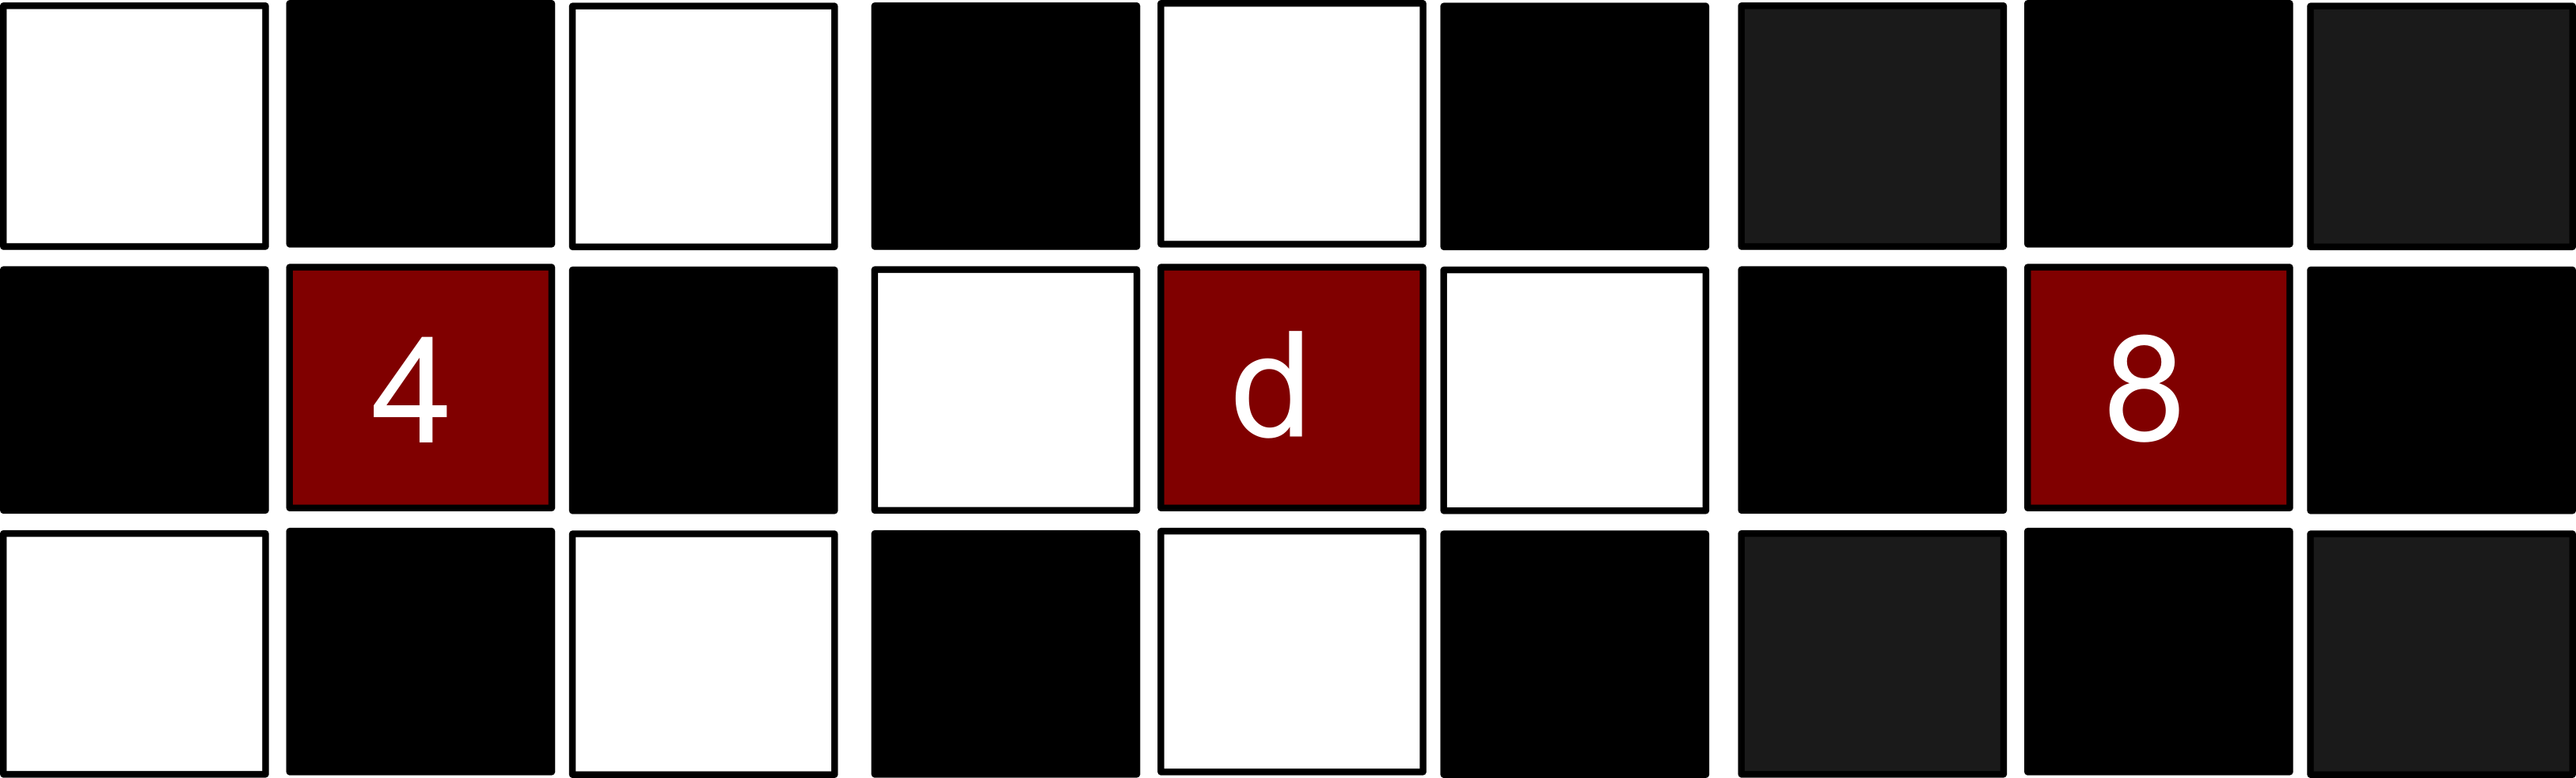
\includegraphics[scale=0.4, bb=0 0 800 200]{imagens/vizinhanca.png}
\end{center}
\caption{(a) 4-vizinhan�a, (b) d-vizinhan�a e (c) 8-vizinhan�a. }
\label{fig:vizinhanca}
\end{figure}



\end{itemize}

Nas pr�ximas subse��es ser�o explicados os principais algoritmos de processamento de imagens implementados no \textit{toolkit} Horus.

\subsection{\textit{Thresholding}}
	O processo de limiariza��o da imagem, tamb�m chamado de \textit{thresholding}, consiste em transformar a imagem que inicialmente se encontra em escala de cinza, com 256 tons diferentes, para uma imagem com apenas dois tons: preto e branco, representados por 0 ou 255 (Figura \ref{fig:imgBin}). No processo de OCR, Essa etapa � utilizada para definir claramente as fronteiras dos caracteres na imagem, afim de prepar�-los para serem analisados pela etapa de extra��o de caracter�sticas.
	Para transformar uma imagem monocrom�tica de 256 tons de cinza em bin�ria podem ser utilizadas t�cnicas de \textit{thresholding} global e adaptativo.
	
\begin{figure}[!htb]
\centering
\begin{center}
    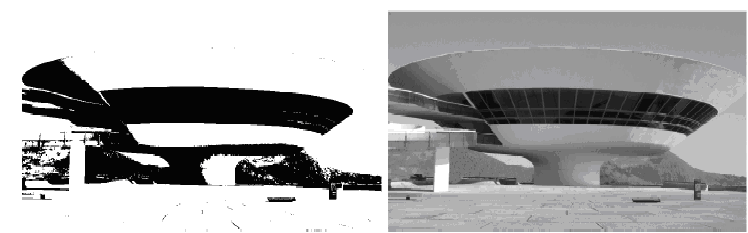
\includegraphics[scale=0.5, bb=0 0 748 233]{imagens/imagemBinaria.PNG}
\end{center}
\caption{Exemplo de imagem bin�ria.}
\label{fig:imgBin}
\end{figure}

\subsubsection{\textit{Thresholding} Global}
\textit{Thresholding} global � um algoritmo simples que depende de um �nico par�metro denominado limiar. O limiar � um valor de intensidade de pixel utilizado como base de compara��o. Sendo assim, em uma imagem monocrom�tica de 256 tons de cinza, todo valor de pixel da imagem de entrada que se encontra abaixo do limiar � colocado como 0 e todo valor acima do limiar � colocado como 255 na imagem resultante.
	Tendo $v$ como o valor do pixel na imagem original e $t$ como limiar, o novo valor de pixel computado �:
	 \[ f(v) = \left\{
                                 \begin{array}{ll}
                                     255,  $ v $ \geq $t$\\
                                     0,  $ v $ \leq $t$
                                 \end{array}
                           \right. \]
	Uma da formas de se obter o valor do limiar \textit{t} � atrav�s de uma inspe��o visual do histograma da imagem. Uma vez que o limiar � utilizado para toda a imagem, o \textit{thresholding} global pode falhar algumas vezes. No caso de imagens com diferen�as de ilumina��o ou parcialmente sombreadas, informa��es que n�o pertencem ao plano de fundo podem ser apagadas. A Figura \ref{fig:thGlobalShadowed} mostra um exemplo de aplica��o de \textit{thresholding} global com imagens sombreadas.

\begin{figure}[!htb]
\centering
\begin{center}
    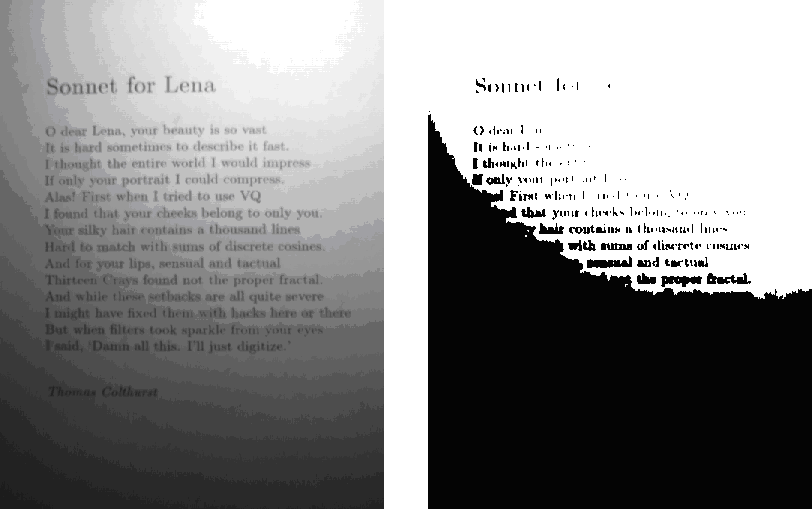
\includegraphics[scale=0.25, bb=0 0 812 509]{imagens/thGlobalShadowed.PNG}
\end{center}
\caption{Imagem original (� direita) e imagem binarizada com thresholding global (� esquerda).}
\label{fig:thGlobalShadowed}
\end{figure}

	Em casos onde a imagem se encontra parcialmente sombreada, a melhor op��o � utilizar a t�cnica de \textit{thresholding} adaptativo.


\subsubsection{\textit{Thresholding} Adaptativo}
No caso de imagens parcialmente sombreadas ou n�o uniformemente iluminadas, o algoritmo de \textit{thresholding} global falha devido � utiliza��o de um �nico limiar para a imagem inteira. Isso pode causar o efeito apresentado na Figura \ref{fig:thGlobalShadowed}. O algoritmo de \textit{thresholding} adaptativo resolve esse problema calculando o limiar para cada pixel da imagem com base na sua vizinhan�a. H� duas abordagens principais de \textit{thresholding} adaptativo: Chow e Kaneko \cite{Chow1972} e \textit{thresholding} local \cite{Gonzales1992}.

\begin{itemize}
\item Abordagem Chow e Kaneko:
 esse m�todo, assim como o de \textit{thresholding} local, se baseia na teoria de que regi�es menores da imagem t�m maior probabilidade de possu�rem uma ilumina��o aproximadamente uniforme. Com isso, o m�todo de Chow e Kaneko divide a imagem em um vetor de sub-imagens sobrepostas e ent�o encontra o limiar �timo para cada sub-imagem atrav�s da an�lise de seus histogramas. O limiar para cada pixel � encontrado interpolando os resultados extra�dos das sub-imagens. Apesar de gerar resultados satisfat�rios, o m�todo de Chow e Kaneko possui um alto custo computacional. Na Figura \ref{fig:chKnk} � mostrado como o limiar de uma subimagem � localizado e a posterior interpola��o dos valores para encontrar o limiar de cada pixel na subimagem.

\begin{figure}[!htb]
\centering
\begin{center}
    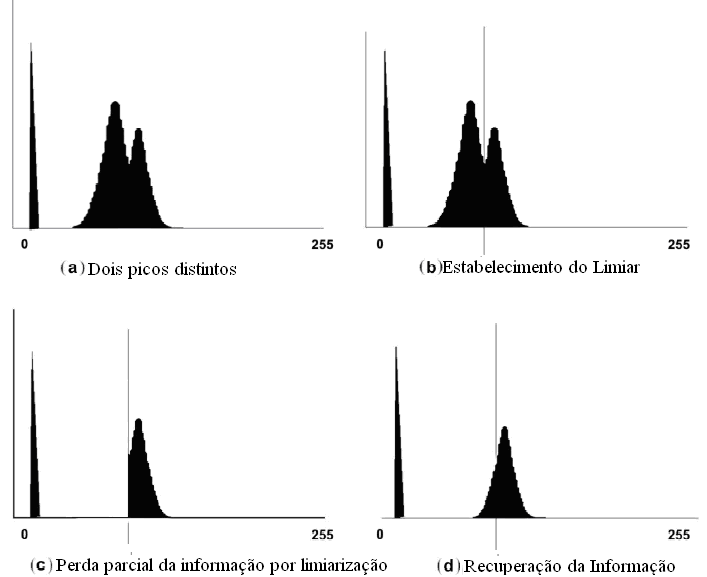
\includegraphics[scale=0.4, bb=0 0 707 577]{imagens/chowAndKaneko.PNG}
\end{center}
\caption{Localiza��o do limiar por Chow e Kaneko.}
\label{fig:chKnk}
\end{figure}

\item \textit{Thresholding} Local:
 a segunda forma de encontrar o limiar de cada pixel � uma inspe��o estat�stica da sua vizinhan�a, levando em considera��o que os vizinhos de um pixel tendem a possuir maior chance de ter uma ilumina��o mais uniforme. No m�todo de \textit{thresholding} local, o limiar de um pixel � definido com base nos valores de um n�mero predeterminado de vizinhos do mesmo. Dessa forma, aplica-se uma opera��o estat�stica nos valores da vizinhan�a de um pixel a fim de obter o seu limiar $t$. Essas opera��es podem ser a m�dia, a mediana ou a m�dia dos valores m�nimo e m�ximo da vizinhan�a. Na Figura \ref{fig:thLocal} � apresentado o c�digo do algoritmo de\textit{thresholding} local, implementado no Horus, utilizando a m�dia entre os valores da vizinhan�a.

\begin{figure}[!htb]
\centering
\begin{center}
    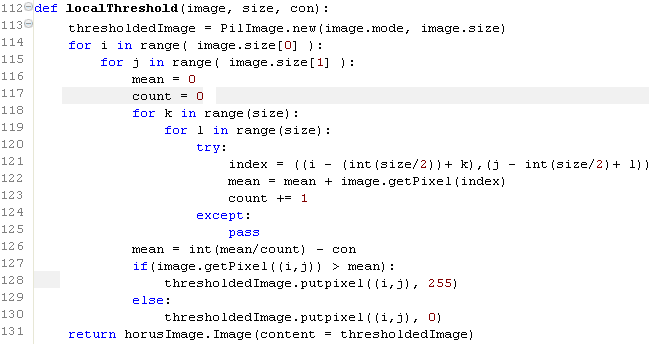
\includegraphics[scale=0.5, bb=0 0 654 344]{imagens/thLocal.PNG}
\end{center}
\caption{C�digo do m�todo de \textit{thresholding} local implementado em linguagem Python.}
\label{fig:thLocal}
\end{figure}
 

No c�digo da Figura \ref{fig:thLocal} os par�metros passados s�o: a imagem (image), o tamanho da vizinhan�a (size) e uma constante que � subtra�da da m�dia (con). Na Figura \ref{fig:imgThLocal} � apresentado o resultado da limiariza��o com o algoritmo de \textit{thresholding} local, utilizando uma vizinhan�a de tamanho $7\times7$ com um valor de constante igual a $7$ ($size = 7$ e $con = 7$).

\begin{figure}[!htb]
\centering
\begin{center}
    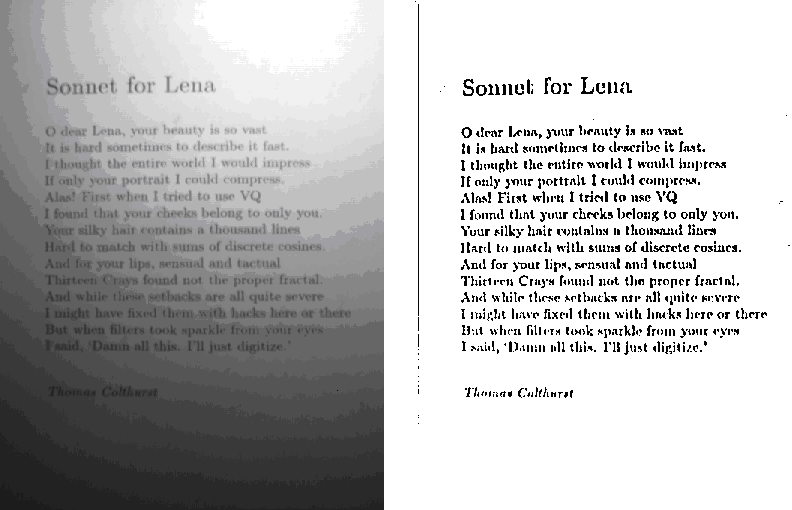
\includegraphics[scale=0.25, bb=0 0 792 510]{imagens/imageThLocal.PNG}
\end{center}
\caption{Imagem original (� direita) e resultado da limiariza��o com \textit{thresholding} local (� esquerda).}
\label{fig:imgThLocal}
\end{figure}


\end{itemize}

\subsection{Skeletonization}

	\textit{Skeletonization} (Esqueletoniza��o) � o processo de remo��o dos pixels de uma imagem, o m�ximo quanto poss�vel, de forma a preservar a estrutura b�sica ou esqueleto da imagem. O esqueleto extra�do deve ser o mais fino quanto poss�vel (largura de um pixel), conectado e centralizado. Quando estas propriedades s�o satisfeitas, o algoritmo deve parar. As Figuras \ref{fig:t_sk} e \ref{fig:b_sk} mostram exemplos de imagens e seus respectivos esqueletos.

\begin{figure}[!htb]
\centering
\begin{center}
    
\includegraphics[scale=0.5, bb=0 0 310 150]{imagens/t_sk.PNG}
\end{center}
\caption{Imagem de um "T" e seu respectivo esqueleto.}
\label{fig:t_sk}
\end{figure}

\begin{figure}[!htb]
\centering
\begin{center}
    
\includegraphics[scale=0.5, bb=0 0 180 224]{imagens/b_sk.PNG}
\end{center}
\caption{Imagem de um "B" (preto) e seu respectivo esqueleto (branco).}
\label{fig:b_sk}
\end{figure}

	Normalmente, o esqueleto de uma imagem enfatiza as propriedades geom�tricas e topol�gicas dos padr�es e � extra�do quando se deseja preservar as caracter�sticas estruturais da imagem, como por exemplo, jun��es, \textit{loops} e termina��es de linha. Essas caracter�sticas podem ser extra�das do esqueleto para serem utilizadas, posteriormente, em um processo de reconhecimento e classifica��o de formas atrav�s de t�cnicas de intelig�ncia computacional.

	O algoritmo de \textit{skeletonization} implementado no Horus utiliza o conceito de "\textit{fire front}". Esse conceito realiza a remo��o iterativa dos pixels da borda dos padr�es at� que as condi��es de conectividade, centraliza��o e espessura do esqueleto sejam satisfeitas. Esse algoritmo, denominado algoritmo de Hilditch, � um processo iterativo em que se aplicam sucessivamente dois passos aos pixels pertencentes � borda de um padr�o. O primeiro passo concentra-se em selecionar os pixels das bordas que ser�o removidos e marc�-los para dele��o. O segundo passo � remover todos os pixels marcados para dele��o no passo anterior. A Figura \ref{fig:grid} ilustra os oito vizinhos do pixel $p_1$.

\begin{figure}[!htb]
\centering
\begin{center}
    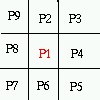
\includegraphics[scale=1, bb=0 0 100 100]{imagens/grid.PNG}
\end{center}
\caption{8-vizinhan�a do pixel $p_1$.}
\label{fig:grid}
\end{figure}

A fim de estabelecer as condi��es para que um pixel da borda seja marcado para dele��o, ser�o definidas duas fun��es:
\begin{itemize}
\item $B(p_1)$: n�mero de vizinhos pretos do pixel $p_1$.
\item $A(p_1)$: n�mero de transi��es de preto para branco $(0$ para $255)$ na seq��ncia $p_2$, $p_3$, $p_4$, $p_5$, $p_6$, $p_7$, $p_8$, $p_9$.
\end{itemize}

\begin{figure}[!htb]
\centering
\begin{center}
    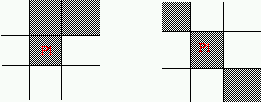
\includegraphics[scale=0.5, bb=0 0 300 150]{imagens/grid2_3.PNG}
\end{center}
\caption{Exemplos das fun��es: (a)$B(p_1)=2$, $A(p_1)=1$  b) $B(p_1)=2$, $A(p_1)=2$.}
\label{fig:grid23}
\end{figure}

A Figura \ref{fig:grid23} mostra exemplos dessas duas fun��es.


H� duas vers�es do algoritmo de Hilditch, uma usando uma janela $4\times 4$ e outra usando uma janela $3\times 3$, nesse trabalho foi utilizada uma janela $3\times 3$. Utilizando as fun��es apresentadas acima, o algoritmo de Hilditch verifica os pixels pretos e marca para dele��o aqueles que satisfazem as quatro seguintes condi��es:

\begin{itemize}
\item $2 \leq B(p_1) \leq 6$: essa condi��o assegura que o n�mero de vizinhos pretos de um pixel seja maior ou igual a 2 e menor ou igual a 6. Isso garante que nenhuma termina��o de linha ou pixel isolado, seja deletada e que o pixel em quest�o seja um pixel de fronteira.

\begin{figure}[!htb]
\centering
\begin{center}
    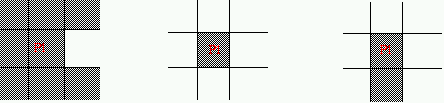
\includegraphics[scale=0.6, bb=0 0 444 103]{imagens/condition1.PNG}
\end{center}
\caption{(a) $B(p_1)=7$ (b) $B(p_1) = 0$ (c) $B(p_1) = 1$.}
\label{fig:condition1}
\end{figure}

	A Figura \ref{fig:condition1} apresenta tr�s condi��es em que um determinado pixel $p_1$ n�o deve ser deletado. Quando $B(p_1)$ � igual a $7$, o pixel n�o � um bom candidato, pois, sua dele��o pode quebrar a conectividade do padr�o. Quando $B(p_1)$ � igual a $1$, significa que o pixel $p_1$ � uma termina��o de linha e j� faz parte do esqueleto, portanto, n�o deve ser removido. Quando $B(p_1)$ � igual a $0$ significa que o pixel $p_1$ � um pixel isolado e tamb�m n�o deve ser removido.

\item $A(p_1) = 1$: essa condi��o representa efetivamente um teste de conex�o. Os casos em que $A(p_1)$ � maior que $1$, a dele��o do pixel $p_1$ causa uma quebra na conectividade do padr�o, como mostra a Figura \ref{fig:condition2}.

\begin{figure}[!htb]
\centering
\begin{center}
    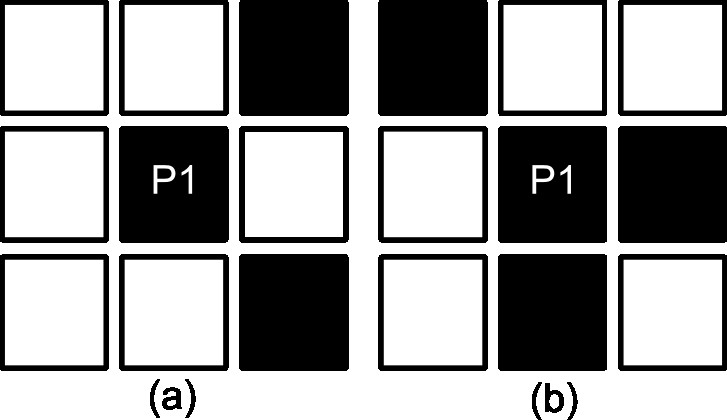
\includegraphics[scale=0.5, bb=0 0 235 104]{imagens/condition2.PNG}
\end{center}
\caption{Exemplos onde $A(p_1)$ � maior que $1$.}
\label{fig:condition2}
\end{figure}

\item $p_2 + p_3 + p_8 \geq 255 $ ou $ A(p_2) \neq 1$: essa condi��o assegura que linhas verticais com largura de dois pixels n�o ser�o inteiramente removidas pelo algoritmo. A Figura \ref{fig:grid11} apresenta uma situa��o em que a condi��o acima � satisfeita.

\begin{figure}[!htb]
\centering
\begin{center}
    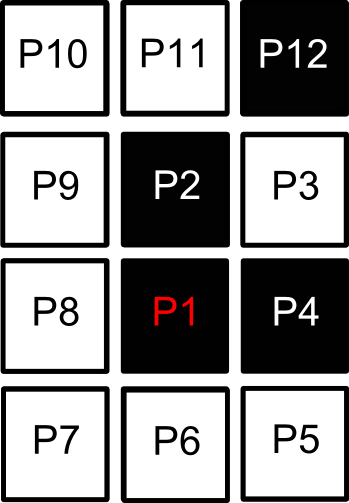
\includegraphics[scale=0.5, bb=0 0 100 130]{imagens/grid11.PNG}
\end{center}
\caption{Exemplo de situa��o em que linhas verticais com largura de dois pixels n�o ser�o inteiramente removidas.}
\label{fig:grid11}
\end{figure}

\item $p_2$ + $p_4$ + $p_6 \geq 255$ ou $A(p_4) \neq 1$: essa condi��o assegura que linhas horizontais com largura de dois pixels n�o ser�o inteiramente removidas pelo algoritmo. A Figura abaixo apresenta uma situa��o em que a condi��o acima � satisfeita.

\begin{figure}[!htb]
\centering
\begin{center}
    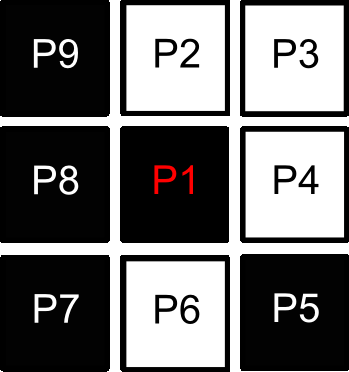
\includegraphics[scale=0.5, bb=0 0 100 100]{imagens/grid13.PNG}
\end{center}
\caption{Exemplo de situa��o em que linhas herticais com largura de dois pixels n�o ser�o inteiramente removidas.}
\label{fig:grid13}
\end{figure}
\end{itemize}

	A cada itera��o do algoritmo, os pixels das bordas s�o analisados, alguns deles s�o marcados para dele��o e ent�o deletados. A Figura \ref{fig:sk_demo} ilustra o processo iterativo do algoritmo, onde, os pixels deletados em cada itera��o s�o representados pelas diferen�as nos tons de cinza da imagem.

\begin{figure}[!Htb]
\centering
\begin{center}
    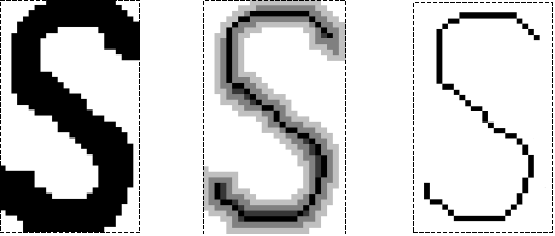
\includegraphics[scale=0.3, bb=0 0 555 236]{imagens/sk_demonstration.PNG}
\end{center}
\caption{(a) padr�o de entrada do algoritmo (b) dele��o iterativa dos pixels das bordas (c) resultado ap�s a execu��o do algoritmo.}
\label{fig:sk_demo}
\end{figure}

O algoritmo de Hilditch � menos custoso do que o algoritmo de transforma��o de eixo mediano. Por�m, esse algoritmo n�o funciona perfeitamente para todos os padr�es. A Figura \ref{fig:erodedPatterns} apresenta dois tipos de padr�es que s�o completamente erodidos pelo algoritmo.

\begin{figure}[!htb]
\centering
\begin{center}
    
\includegraphics[scale=0.4, bb=0 0 337 154]{imagens/erodedPatterns.PNG}
\end{center}
\caption{Padr�es completamente erodidos pelo algoritmo de Hilditch.}
\label{fig:erodedPatterns}
\end{figure}

\section{Vis�o}

	O Sistema de Vis�o � um dos mais complexos e completos do ser humano, pois fornece um conjunto de informa��es necess�rias � intera��o do homem com o ambiente. Tal processo se inicia com a capta��o dos est�mulos luminosos do ambiente formando uma imagem, que juntamente aos outros est�mulos captados por demais sensores do corpo (som, temperatura, press�o, umidade, cheiro, etc) e as informa��es contidas na mem�ria, comp�em uma cena compreendida pelo c�rebro.

	Esse m�dulo tem como principal objetivo o reconhecimento de padr�es.	Na aplica��o Ariadnes, desenvolvida neste trabalho, o padr�o a ser reconhecido � uma placa com o nome dos locais do ambiente e setas que indicam as dire��es dos mesmos. Para reconhecimento de uma placa � necess�rio identificar algumas caracter�sticas de uma imagem, que servir�o de padr�es de entrada para uma rede neural. 

\subsection{Extra��o de caracter�sticas}
\label{section:features}
	Para realizar o reconhecimento de objetos em uma cena, � necess�rio extrair caracter�sticas das imagens desse objeto, de forma a identific�-lo, independentemente das varia��es com que ele possa ocorrer na imagem. O 
\textit{toolkit} Horus apresenta alguns algoritmos para extra��o de caracter�sticas, os principais deles ser�o explicados nos itens abaixo.
\begin{itemize}
\item Matriz de Pixel: a maneira mais simples de extrair caracter�sticas de um \textit{bitmap} � associar a lumin�ncia de cada pixel com um valor num�rico correspondente no vetor de caracter�sticas. 

   Esse m�todo, apesar de simples, possui alguns problemas que podem torn�-lo inadequado para o reconhecimento de caracteres. O tamanho do vetor � igual � altura do \textit{bitmap} multiplicado pela sua largura, portanto, \textit{bitmaps} grandes produzem vetores de caracter�sticas muito longos, o que n�o � muito adequado para o reconhecimento. Logo, o tamanho do \textit{bitmap} � uma restri��o para esse m�todo. Al�m disso, este m�todo n�o considera a proximidade geom�trica dos pixels, bem como suas rela��es com a sua vizinhan�a. No entanto, este m�todo pode ser adequado em situa��es onde o \textit{bitmap} do caractere se encontra muito opaco ou muito pequeno para a detec��o de arestas. 
            
            
 \begin{figure}[!htb]
\centering
\begin{center}
    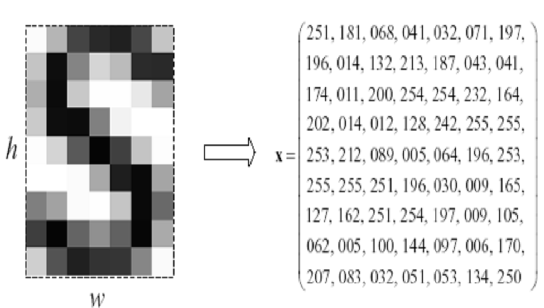
\includegraphics[scale=0.3, bb= 0 0 559 310]{imagens/pixelMatrix.PNG}
\end{center}
\caption{Matriz de pixel de um \textit{bitmap}.}
\label{fig:seg}
\end{figure}
            
            
\item Histograma de Arestas por Regi�es: esse m�todo extrai o n�mero de ocorr�ncias de determinados tipos de arestas em uma regi�o espec�fica do \textit{bitmap}. Isso torna o vetor de caracter�sticas desse m�todo invariante com rela��o � disposi��o das arestas em uma regi�o e a pequenas deforma��es do caractere. Sendo o \textit{bitmap} representado pela fun��o discreta $f (x, y)$, largura $w$ e altura $h$, onde $0 \leq x < w$ e $0 \leq y < h$. Primeiramente � realizada a divis�o do \textit{bitmap} em seis regi�es $(r_0, r_1, ..., r_5)$ organizadas em tr�s linhas e duas colunas. Outros quatro layouts podem ser utilizados para a divis�o do \textit{bitmap} em regi�es.

\begin{figure}[!htb]
\centering
\begin{center}
    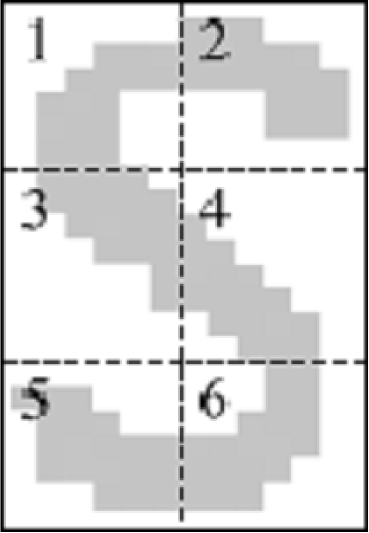
\includegraphics[scale=0.2, bb= 0 0 394 556]{imagens/layoutsix.PNG}
\end{center}
\caption{Layout com seis regi�es em tr�s linhas e duas colunas.}
\label{fig:seg2}
\end{figure}

Definindo a aresta de um caractere como uma matriz $2\times2$ de transi��es de branco para preto nos valores dos pixels, t�m-se quatorze diferentes tipos de arestas, como ilustrado na Figura \ref{fig:seg4}.

\begin{figure}[!htb]
\centering
\begin{center}
   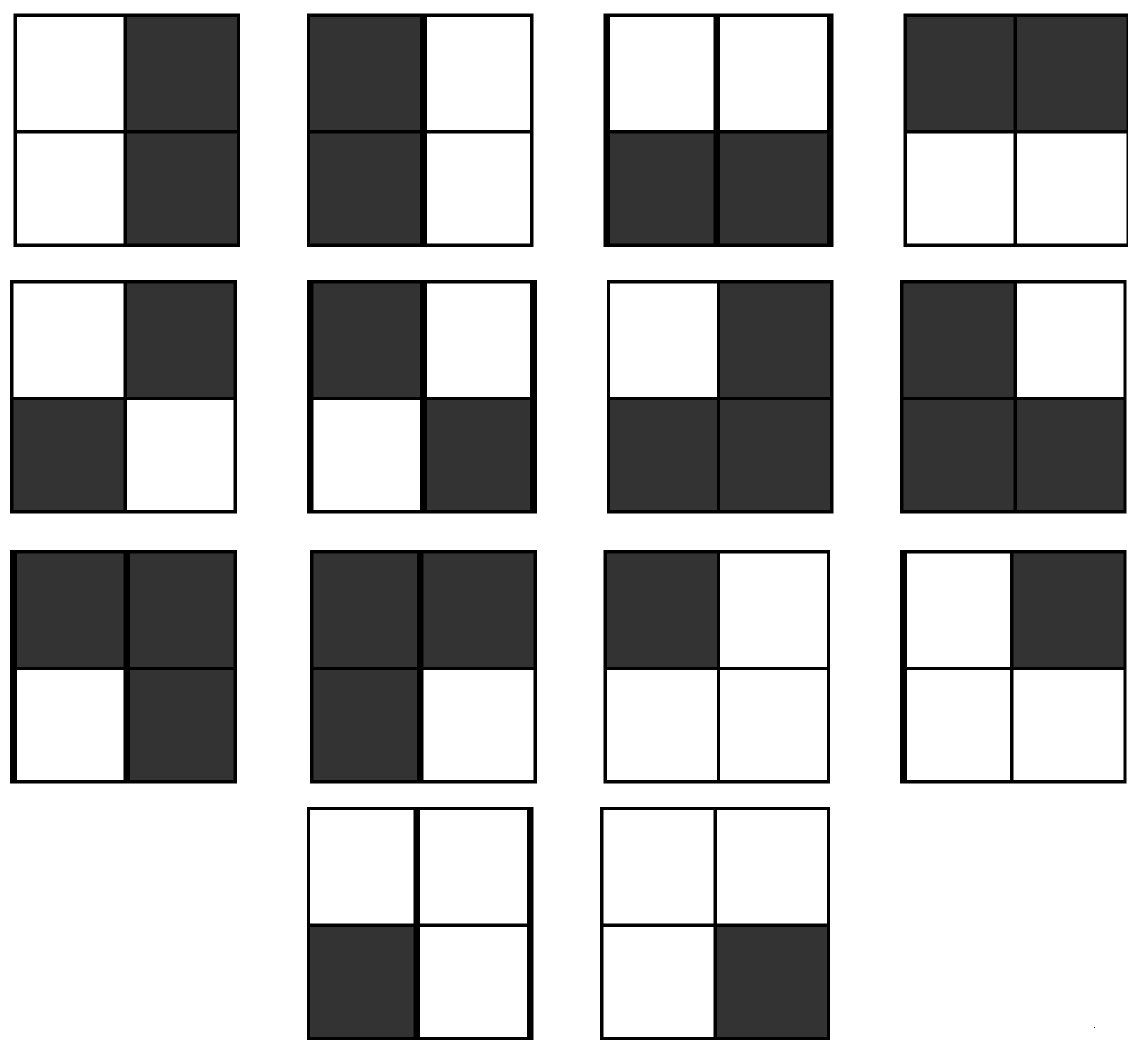
\includegraphics[scale=0.2, bb= 0 0 800 700]{imagens/quatorze.PNG}
\end{center}
\caption{Quatorze diferentes tipos de arestas.}
\label{fig:seg4}
\end{figure}



O vetor de ocorr�ncias de cada tipo de aresta em cada sub-regi�o da imagem � normalmente muito longo o que n�o � uma boa pr�tica em reconhecimento de padr�es, onde o vetor de caracter�sticas deve ser t�o menor quanto poss�vel. Com isso, pode-se agrupar tipos de arestas semelhantes para reduzir o tamanho do vetor de caracter�sticas. Por quest�es de simplicidade, o agrupamento dos tipos de aresta ser� desconsiderado no algoritmo de extra��o de caracter�sticas. Sendo $n$ igual ao n�mero de tipos de arestas diferentes, onde $h_{i}$ � uma matriz $2\times2$  que corresponde ao tipo espec�fico de aresta, e $p$ igual ao n�mero de regi�es retangulares em um caractere t�m-se:


 \begin{figure}[!htb]
\centering
\begin{center}
    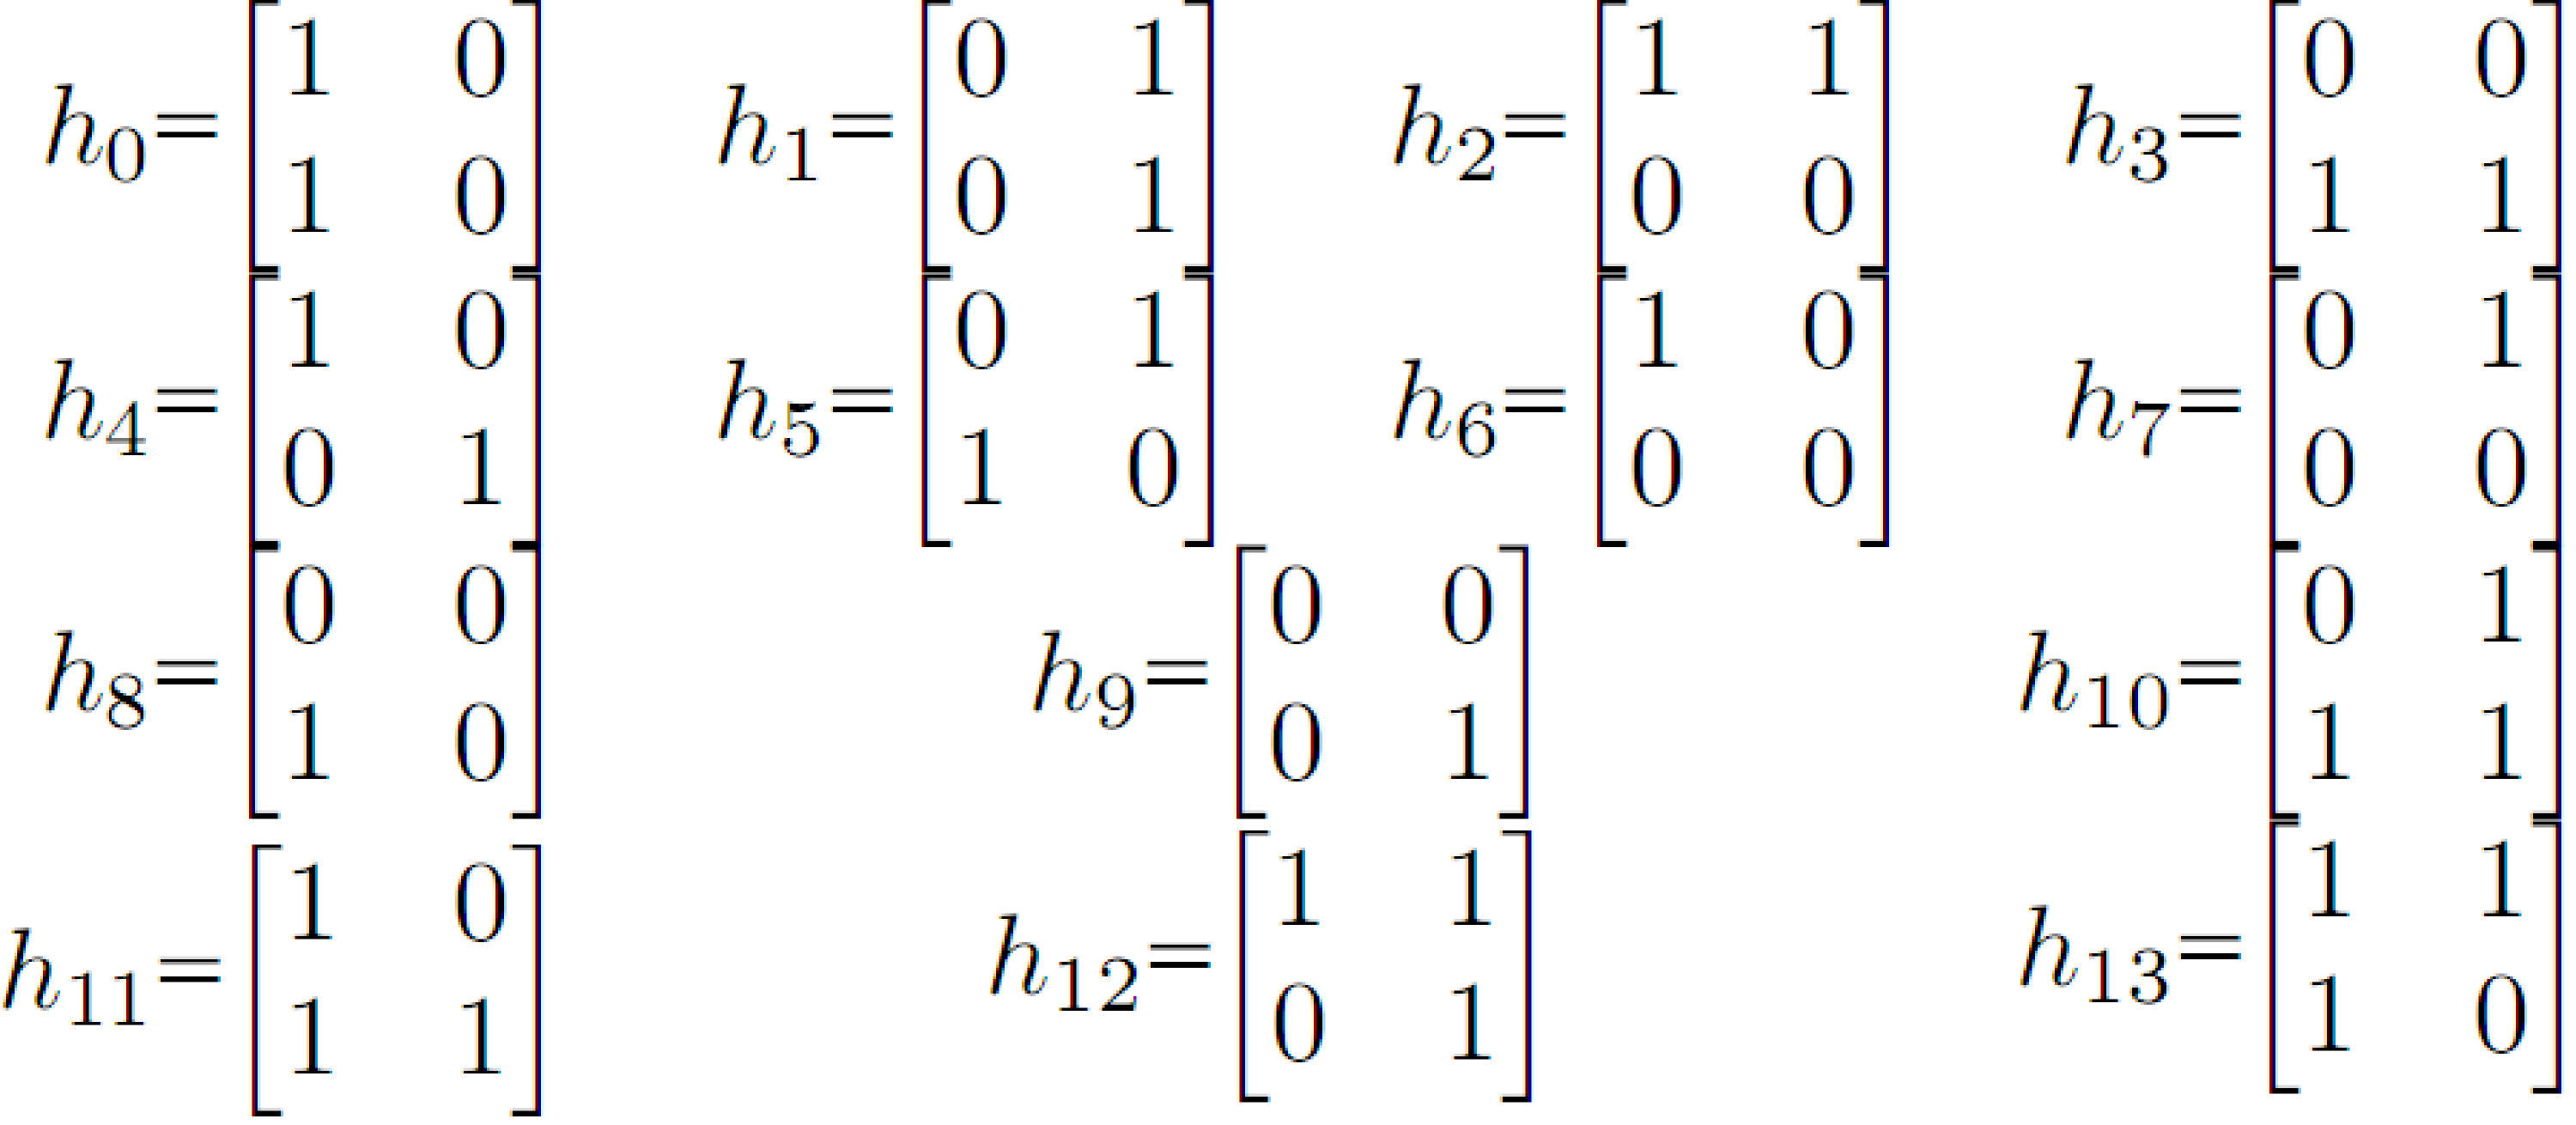
\includegraphics[scale=0.4, bb= 0 0 600 300]{imagens/matriz.PNG}
\end{center}
\caption{Matrizes referentes aos tipos de arestas.}
\label{fig:matriz}
\end{figure}

O vetor de caracter�sticas de sa�da � ilustrado pelo padr�o abaixo. A nota��o $h_j@r_i$ siginifica "n�mero de ocorr�ncias de um tipo de aresta representado pela matriz $h_j$ na regi�o $r_i$", \ref{fig:vetor} 


\begin{figure}[!Htb]
\centering
\begin{center}
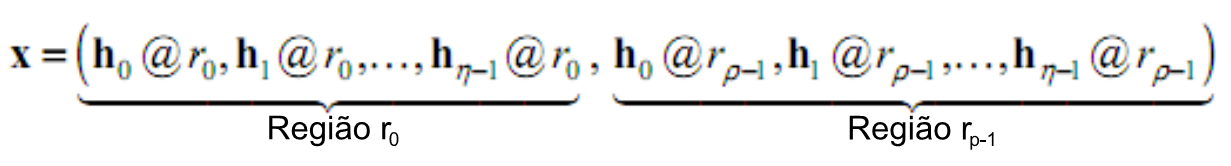
\includegraphics[scale=0.6
, bb= 0 0 500 166]{imagens/vetorCaracteristicas.PNG}
\end{center}
\caption{Vetor de Caracter�sticas.}
\label{fig:vetor}
\end{figure}

\end{itemize}


Uma outra forma de extra��o de caracter�sticas � a an�lise estrutural do padr�o. Atrav�s desse tipo de extra��o � poss�vel diferenciar padr�es por suas caracteristias mais substanciais. No caso de reconhecimento de caracteres, a an�lise estrutural leva em considera��o estruturas mais complexas, como jun��es, termina��o de linha e \textit{loops}.

\begin{itemize}
\item Termina��o de Linha: � representada por um ponto que possui exatamente um vizinho de pixel preto na 8-vizinhan�a.   
   
\item Jun��es: consiste em um ponto que possui pelo menos tr�s pixels pretos na 8-vizinhan�a. No presente trabalho, considerou-se apenas dois tipos de jun��es: com tr�s e quatro vizinhos. A Figura 000000 mostra um exemplo de cada caso.

\item \textit{Loops}: esta � a caracter�stica estrutural mais complexa de ser extra�da em um caractere. Neste trabalho, o processo de contagem de \textit{loops} trabalha com a imagem negativa do caractere (Figura 00000), ou seja, o fundo da imagem � representado pela cor preta, enquanto que o caractere � representado pela cor branca. O n�mero de loops pode ser calculado como o n�mero de grupos de pixels pretos na imagem negativa, representado na Figura 00000 pelos n�meros 1, 2, 3, subtraido de um. Essa subrta��o � feita para desconsiderar o fundo da imagem como um \textit{loop}.
\end{itemize} 

O \textit{toolkit} Horus tamb�m fornece algumas implementa��es de algoritmos para an�lise estrututal de caracteres.

\subsection{Reconhecimento de Objetos}
	Reconhecimento de objetos � o processo de identifica��o de um determinado objeto atrav�s de suas caracter�sticas. Normalmente, esse processo se inicia com a captura de informa��es sobre o objeto atrav�s de c�meras ou outros tipos de sensores, como sonares por exemplo. Em seguida, essas informa��es passam pelo processo de extra��o de caracter�sticas com a finalidade de se extrair um vetor de informa��es que identifique unicamente o objeto independente das varia��es  que ele possa apresentar. Por fim, esse vetor de caracter�sticas � passado para o processo de reconhecimento, o qual identifica o objeto atrav�s de suas caracter�sticas.

	Para tarefas de reconhecimento, o Horus disponibiliza fun��es para constru��o e treinamento de redes neurais atrav�s da utiliza��o de uma biblioteca denominada FANN (\textit{Fast Artificial Neural Network}). O FANN � uma biblioteca de c�digo aberto implementada em linguagem C que fornece conectores para diversas linguagems de alto n�vel, dentre elas pode-se citar: Java, C++, Python e Ruby.

	Outra funcionalidade disponibilizada pelo Horus para reconhecimento de objetos � o m�dulo de OCR. Esse m�dulo utiliza uma engine OCR \textit{Open Source} chamada de Tesseract. Essa engine est� sob a licensa Apache e � escrita nas linguagens de programa��o C e C++. O m�dulo OCR do Horus pode ser utilizado em aplica��es em que haja a necessidade de se reconhecer textos existentes em imagens. 	       

	O m�dulo OCR � utilizado nas aplica��es ANPR e Ariadnes. No ANPR, esse m�dulo  � utilizado para reconhecer o texto que se encontra nas placas dos autom�veis. J� na aplica��o Ariadnes, o agente inteligente utiliza esse m�dulo para reconhecer os textos que se encontram nas placas informativas presentes no ambiente.
	
\section{Mapeamento e Navega��o}
\label{sec:slam}
 Chamamos de mapeamento o processo de identificar locais no ambiente do simulador e representa-los em um grafo. O mapeamento no Horus utiliza uma t�cnica gen�rica denominada SLAM. Nessa t�cnica, um agente consegue realizar o mapeamento e a localiza��o no ambiente de forma simult�nea. Os dispositivos utilizados pela implementa��o da t�cnica SLAM s�o lasers,  para identificar obst�culos, e um od�metro, para medir dist�ncias percorridas.
 
	O SLAM � composto por v�rios procedimentos interligados. Cada um desses procedimentos pode ser implementado de diversas formas. Dentre os procedimentos implementados no Horus, podemos citar:

\begin{enumerate}
	\item \textit{Landmark Extraction}: procedimento respons�vel pela extra��o de marcos no ambiente.
	\item \textit{Data Association}: procedimento que associa os dados extra�dos de um mesmo marco por diferentes leituras de lasers.
	\item \textit{State Estimation}: procedimento respons�vel por estimar a posi��o atual do rob� com base em seu od�metro e nas extra��es de marcos no ambiente.
	\item \textit{State Update}: procedimento que atualiza o estado atual do agente.
	\item \textit{Landmark Update}: procedimento que atualiza as posi��es dos marcos no ambiente em rela��o ao agente. 
\end{enumerate}

  Neste trabalho, a proposta utilizada � mapear o ambiente atrav�s de um grafo conexo, cujos n�s referem-se a: entradas/sa�das do ambiente, acessos aos c�modos, obst�culos fixos e esquinas. O peso das arestas � calculado de acordo com o custo de processamento no deslocamento entre a posi��o de um n� ao outro. 

  O problema de navega��o consiste na localiza��o e defini��o do caminho que o agente deve seguir. Ap�s a constru��o de uma representa��o do ambiente em forma de um grafo, o agente � capaz de se localizar e se movimentar pelo ambiente atrav�s dos v�rtices e arestas, previamente mapeados no grafo. Para a utiliza��o de grafos, o Horus fornece classes para sua constru��o e algoritmos para c�lculo de caminho m�nimo.

\chapter{Ariadnes}
\label{cap:ariadnes}

Ariadnes � um sistema que simula a navega��o e movimenta��o aut�noma de um agente inteligente em um ambiente completamente desconhecido. Inicialmente o agente tem o objetivo de chegar a uma determinada sala no ambiente utilizando t�cnicas de localiza��o e mapeamento de ambientes e de vis�o computacional. Da mesma forma que o Teseu, apresentado na Se��o \ref{sec:app}, o ambiente e atores do Ariadnes foram modelados utilizando Blender e s�o manipulados utilizando o Panda3D.

Esse simulador � composto por quatro partes principais baseadas no \textit{toolkit} Horus. A Figura \ref{fig:arquiteturaAriadnes} apresenta a arquitetura conceitual do simulador Ariadnes com seus principais componentes.

\begin{figure}[!htb]
\centering
\begin{center}
 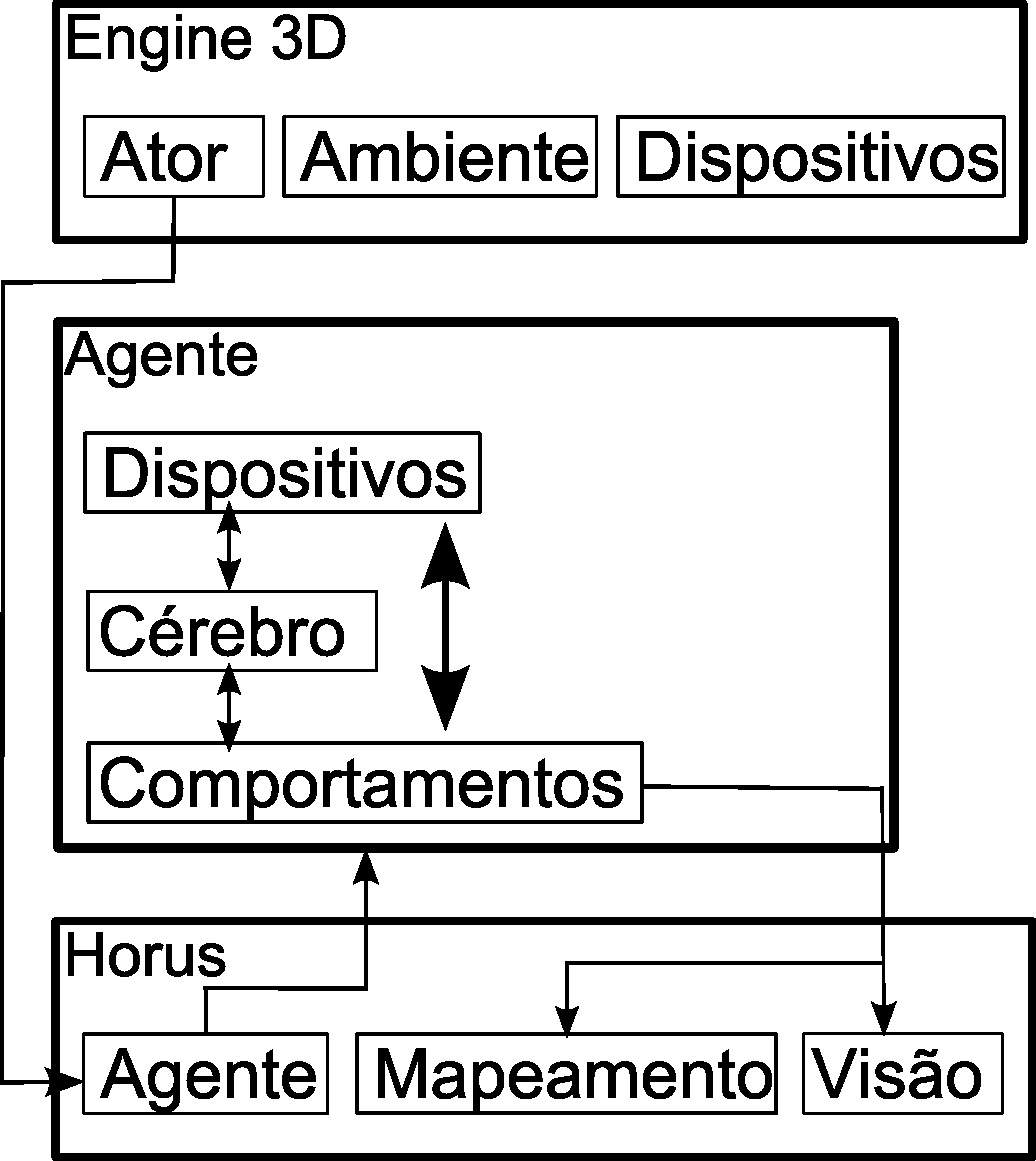
\includegraphics[scale=0.15, bb=0 0 1036 1161]{imagens/arquiteturaAmbiente.png}
\end{center}
\caption{Arquitetura conceitual do simulador Ariadnes.}
\label{fig:arquiteturaAriadnes}
\end{figure}


 \begin{figure}[!htb]
\centering
\begin{center}
    
\includegraphics[scale=0.3, bb=0 0 761 408]{imagens/placa.PNG}
\end{center}
\caption{Placa informativa presente no ambiente.}
\label{fig:placa}
\end{figure}

As principais partes do simulador Ariadnes s�o: ambiente, engine 3D, agentes e dispositivos. O ambiente, nesse simulador,  � composto basicamente de diversos c�modos interligados por corredores, em alguns pontos desse ambiente existem placas informativas cujo objetivo � orientar o agente durante o mapeamento, como mostra a Figura \ref{fig:placa}. 

\begin{figure}[!htb]
\centering
\begin{center}
    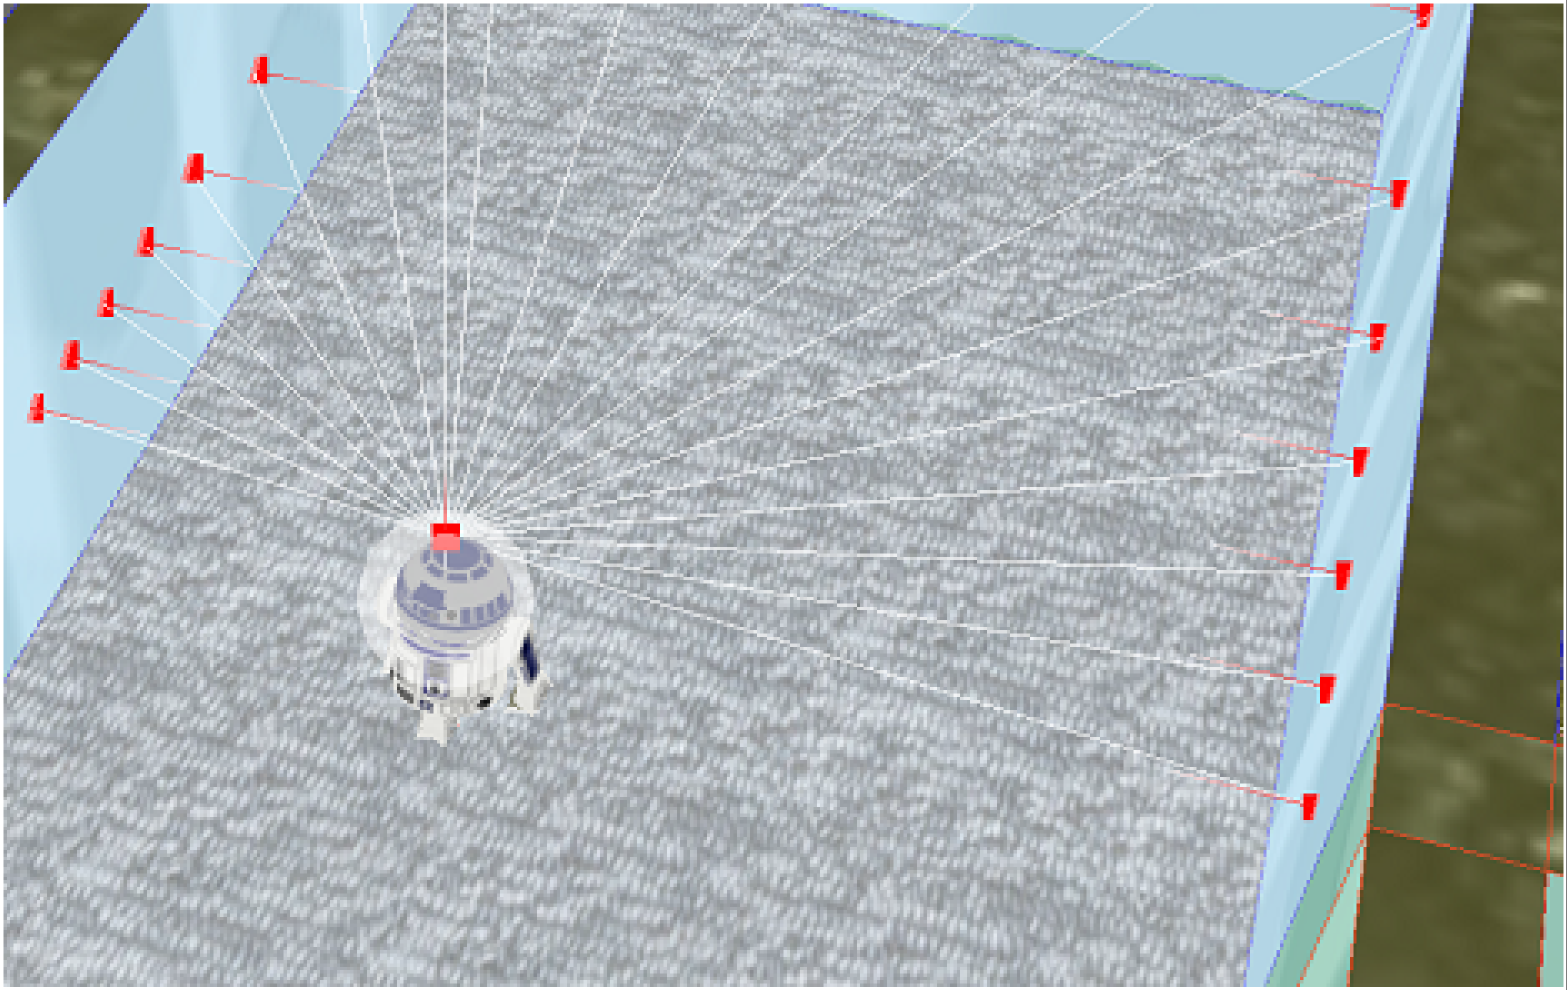
\includegraphics[scale=0.2, bb=0 0 1567 990]{imagens/robo.png}
\end{center}
\caption{Agente configurado com dispositivos de lasers.}
\label{fig:lasers}
\end{figure}

 Por �ltimo, agentes e dispositivos s�o extens�es de abstra��es fornecidas no m�dulo \textit{Core} do Horus para implementa��o de tais partes. O agente configurado com dispositivos emissores de lasers � mostrado na Figura \ref{fig:lasers}.

\begin{figure}[!htb]
\centering
\begin{center}
    \includegraphics[scale=0.2, bb=0 0 566 724]{imagens/galpao.png}
\end{center}
\caption{Ambiente utilizado no Ariadnes.}
\label{fig:ambiente}
\end{figure}

Inicialmente, o agente � configurado com os comportamentos de Navega��o, Mapeamento, Localiza��o e Leitura de placas. Ap�s a configura��o, o agente � inserido em um ambiente totalmente desconhecido com a miss�o de chegar a uma sala espec�fica. Na Figura \ref{fig:ambiente} � apresentado a vista superior do ambiente utilizado no Ariadnes.


Ap�s o estabelecimento da miss�o, o agente inicia o mapeamento do ambiente utilizando os algoritmos do m�dulo Mapeamento do Horus para construir uma representa��o do ambiente em forma de grafo. 

A m�quina de estados utilizada no Ariadnes � composta por: mapeamento, navega��o, reconhecimento de objetos e execu��o. O agente tem por objetivo partir de um ponto inicial para um ponto final, para isso, ele tenta definir uma rota. Nesse momento, o agente se encontra no estado de navega��o. Caso ele n�o consiga definir uma rota, o estado desse agente muda para mapeamento. Nesse estado, ele explorar� o ambiente at� que encontre uma placa ou algum ponto j� mapeado. Caso encontre a placa, seu estado mudar� para reconhecimento de objetos. Nesse estado, caso a placa seja a identifica��o do c�modo destino, seu estado muda para execu��o. Caso contr�rio, o agente muda para o estado de navega��o ou retorna para o estado de reconhecimento de objetos, caso a placa identificada seja informativa. No estado de execu��o, uma tarefa espec�fica, previamente determinada, � realizada. No estado de mapeamento, ao encontrar um ponto j� mapeado, ele verifica se agora � poss�vel tra�ar uma rota at� seu objetivo. Caso n�o seja poss�vel, o agente continua no estado de mapeamento.
O agente � capaz de estimar sua posi��o local para se localizar globalmente e recuperar-se de poss�veis erros de localiza��o. A proposta utilizada para realiza��o das etapas de mapeamento e localiza��o � a t�cnica SLAM, descrita na Se��o \ref{sec:slam}. Durante o mapeamento, uma c�mera � utilizada pelo agente para localizar as placas informativas presentes no ambiente. Quando este depara-se com uma dessas placas, interrompe o processo de mapeamento e utiliza algoritmos de vis�o para interpretar o conte�do existente na placa, a fim de estabalecer a dire��o para a qual ele deve seguir no ambiente. A captura da cena por c�meras permite a utiliza��o de procedimentos de vis�o computacional, como extra��o de caracter�sticas, OCR, localiza��o de placas e reconhecimento de informa��es de dire��o presentes no ambiente. No ambiente utilizado no Ariadnes existem marcos, localizados no ch�o, com os objetivos de: auxiliar a localiza��o das placas identificadoras de c�modos e dire��es e diminuir o tempo necess�rio no processo de localiza��o das placas. Para isso, o agente � configurado com duas c�meras: uma delas apontando para o ch�o, utilizada para localizar os marcos no ch�o do ambiente; e a segunda c�mera � apontada para frente do agente, simulando sua vis�o, essa c�mera � utilizada no processo de localiza��o e reconhecimento das placas. A Figura \ref{fig:cameras} mostra uma foto capturada por cada uma das c�meras citas.

            
\begin{figure}[!htb]
\centering
\begin{center}
    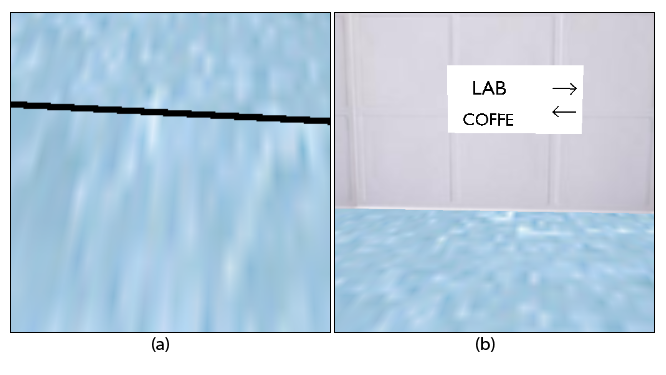
\includegraphics[scale=0.4, bb= 0 0 666 375]{imagens/cameras.png}
\end{center}
\caption{Imagens capturadas no ambiente pelas c�meras do rob� (a) C�mera para baixo.  (b) C�mera frontal. }
\label{fig:cameras}
\end{figure}

  Ao encontrar um marco, (FALAR do ALINHAMENTODO ROBO ANTES DE FOTOGRAFAR) o agente fotografa a placa. Com essa imagem, inicia-se o processo de reconhecimento da placa. Esse processo consiste nas etapas de: localiza��o e segmenta��o da placa, distin��o de setas e textos, reconhecimento do texto, identifica��o da dire��o da seta.
  O processo de localiza��o da placa pode ser resolvido em duas etapas. A primeira etapa consiste em localizar a regi�o da placa na imagem. Inicialmente, aplica-se o filtro de Sobel, a fim de detectar as arestas horizontais e verticais. Ap�s a detec��o das arestas, pretende-se encontrar a regi�o com maior densidade de arestas, pois, geralmente a placa se encontra nessa regi�o. Esse processo � analogo a localiza��o de placas descrito na Se��o \ref{cap:anpr}.

A placa � constitu�da de v�rias linhas, cada linha cont�m duas colunas. A primeira coluna de cada linha fornece o nome de um determinado local no ambiente, enquanto que, a segunda coluna fornece a dire��o desse local em forma de setas. Como apresentado na Figura \ref{fig:placa}.

Para realizar o reconhecimento dos locais e dire��es apresentados na placa, � necess�rio uma etapa de segmenta��o dessa placa em duas regi�es, textos e dire��es. Para isso, aplica-se a proje��o horizontal para identificar cada regi�o, a Figura \ref{fig:corte_horizontal} mostra o resultado da proje��o horizontal na imagem da placa. 

\begin{figure}[!htb]
\centering
\begin{center}
    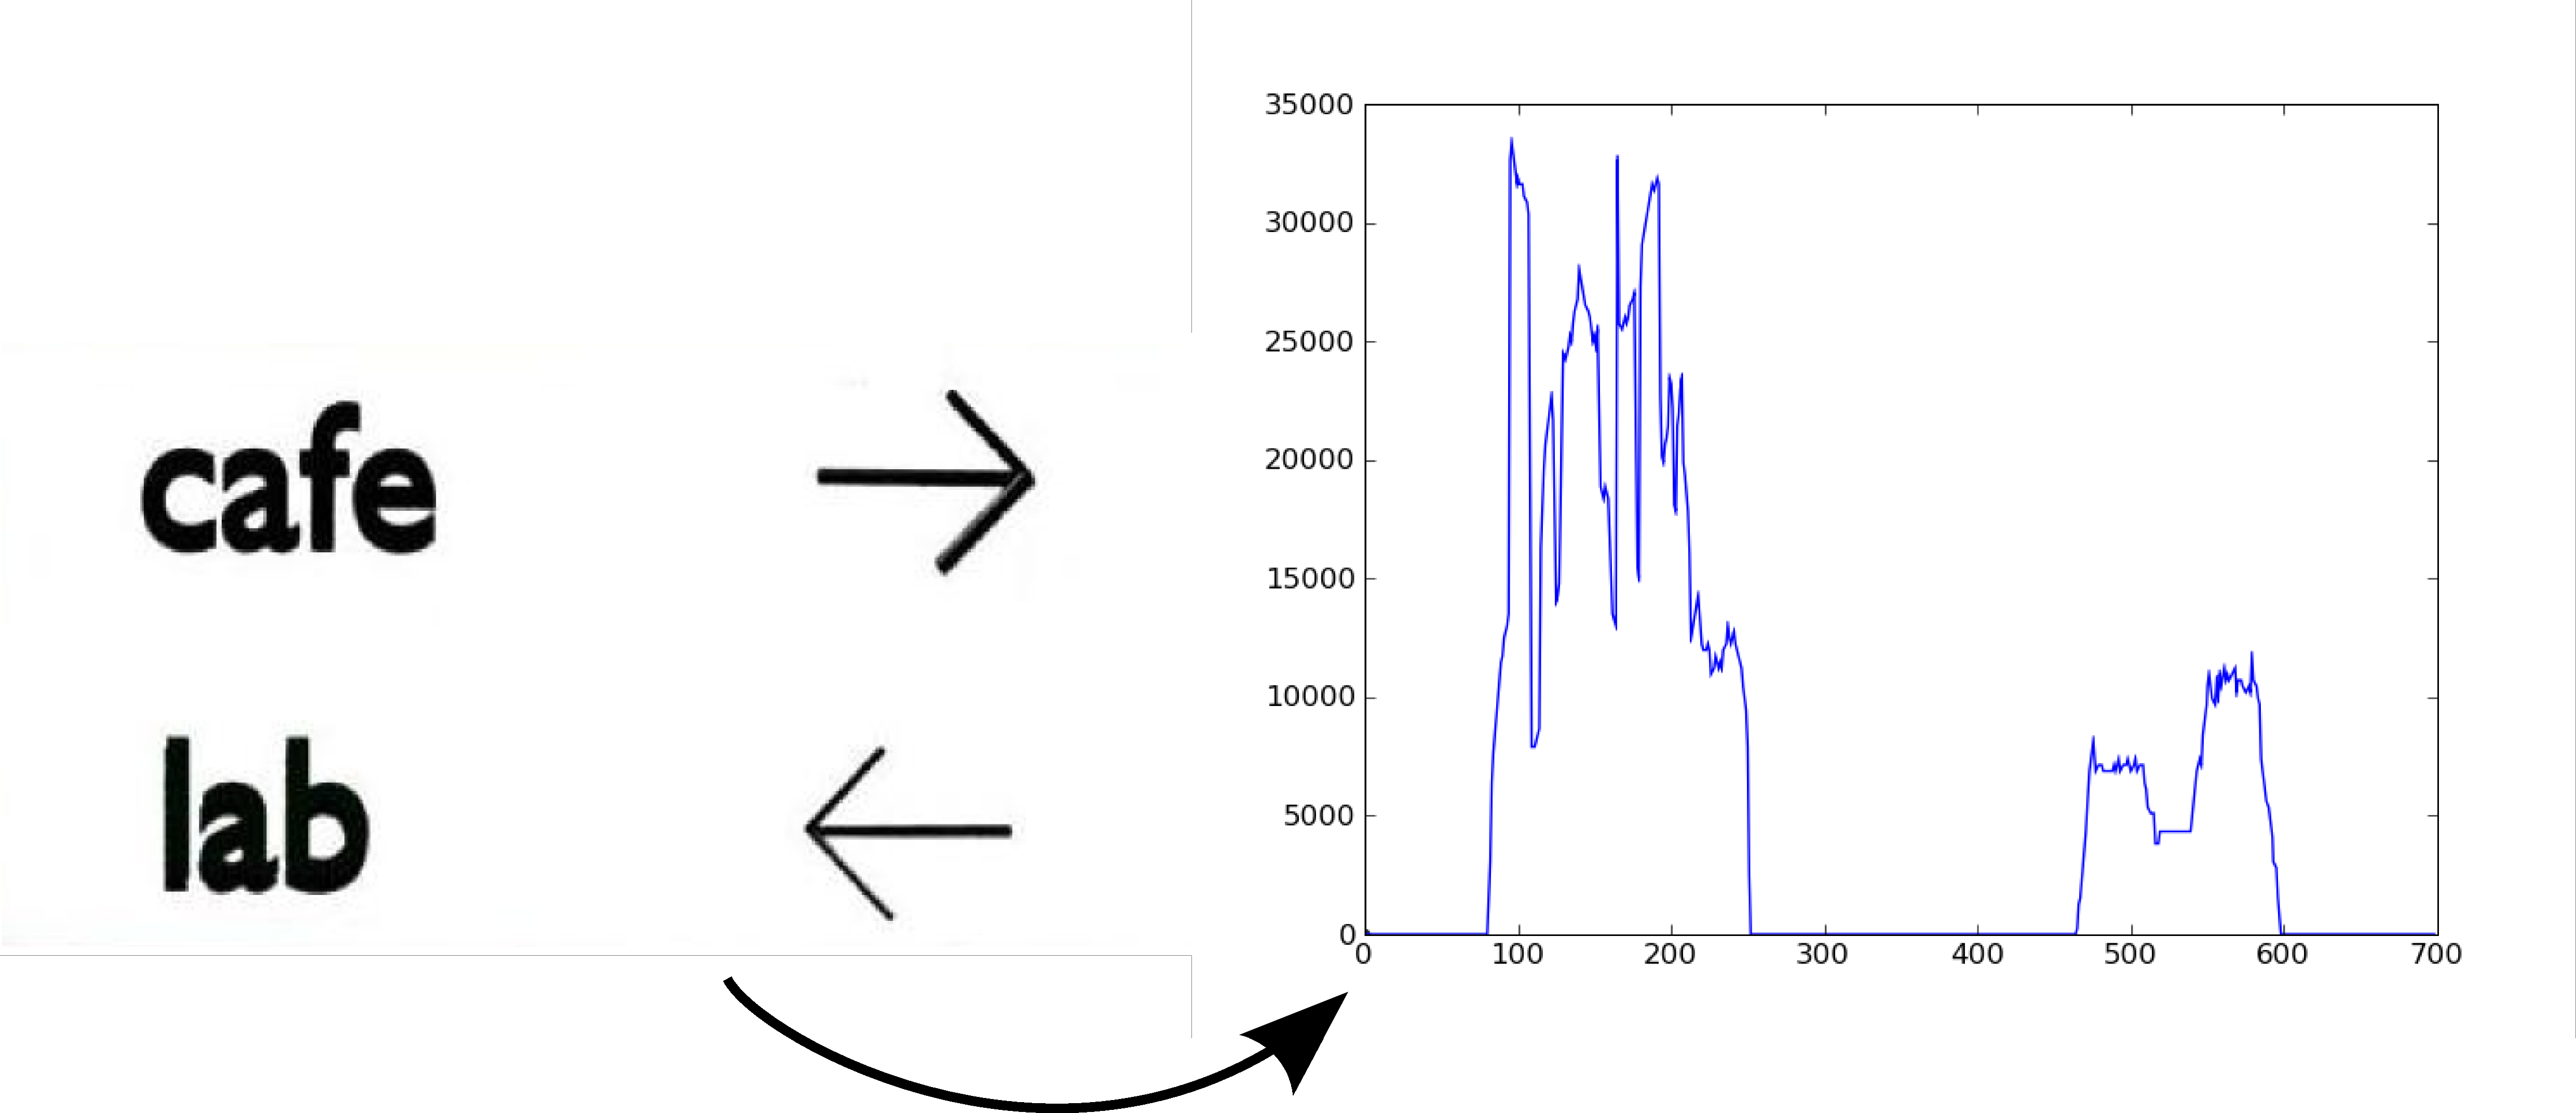
\includegraphics[scale=0.2, bb=0 0 1000 500]{imagens/corte_horizontal.png}
\end{center}
\caption{Proje��o horizontal de uma placa informativa.}
\label{fig:corte_horizontal}
\end{figure}


Ap�s a etapa de segmenta��o da imagem em duas regi�es, separa-se cada coluna em linhas. Isso � feito atrav�s da proje��o vertical, como mostra a Figura \ref{fig:corte_vertical}

 \begin{figure}[!htb]
 \centering
 \begin{center}
     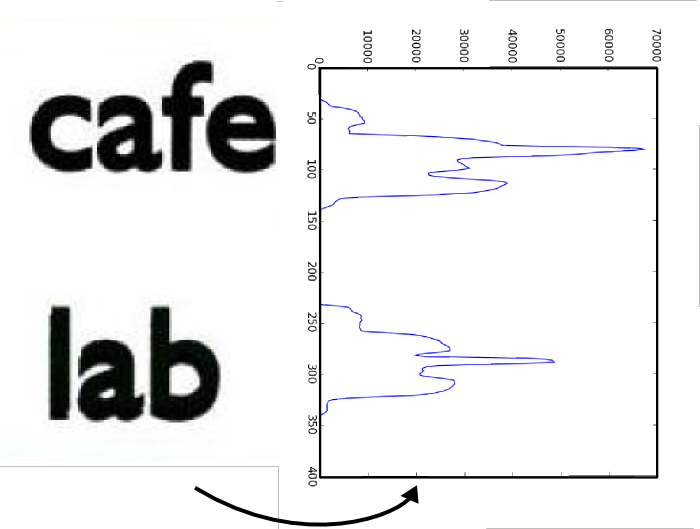
\includegraphics[scale=0.2, bb=0 0 700 529]{imagens/corte_vertical.png}
 \end{center}
 \caption{Proje��o vertical das colunas da placa.}
 \label{fig:corte_vertical}
 \end{figure}

 Para a identifica��o do texto e da seta de cada linha, utiliza-se os m�todos de extra��o de caracter�sticas do Horus, utilizando-os para cria��o dos vetores de caracter�ticas que servir�o como padr�es de entrada para uma rede neural artificial, tamb�m implementada no Horus. Por fim, o agente identifica os locais e suas respectivas dire��es, presentes na placa, e define a dire��o para qual ele deve seguir baseado em seu objetivo pr�-estabelecido.

%%%%%%%%%%%%%%%%%%%%%%%%%%%%%%%%%%%%%
%%  ANPR

%%%%%%%%%%%%%%%%%%%%%%%%%%%%%%%%%%%%%

\chapter{PyANPR}
\label{cap:anpr}

  Nesse cap�tulo ser�o abordados os principais conceitos sobre um sistema de Reconhecimento Autom�tico de N�meros de Placas (\textit{Automatic Number Plate Recognition} - ANPR). Nesse trabalho ser� adotado o acr�nimo do termo em ingl�s ANPR. Atualmente, ANPR se tornou a principal t�cnica para muitos sistemas de transporte automatizado, como monitoramento de tr�fego em estradas, pagamento autom�tico de ped�gios e controle de acesso a pontes e estacionamentos. Esse tipo de sistema consiste em, a partir de uma imagem de um carro, localizar a placa e identificar os caracteres presentes nesta. Com base no reconhecimento dos caracteres presentes na placa, � poss�vel identificar o carro e levantar informa��es sobre o mesmo automaticamente.

    Sistemas ANPR tamb�m s�o conhecidos como: \textit{Automatic licence plate recognition} (ALPR), \textit{Automatic vehicle identification} (AVI), \textit{Car plate recognition} (CPR), \textit{Licence plate recognition} (LPR) e \textit{Lecture Automatique de Plaques d'Immatriculation} (LAPI). A id�ia de um sistema ANPR foi criado em 1976, pelo Departamento de Desenvolvimento Cient�fico da Pol�cia no Reino Unido, com o objetivo de identificar carros roubados. O primeiro prot�tipo desenvolvido, ficou pronto em 1979, e foi desenvolvido pela empresa Brit�nica EMI \textit{Electronics}. Esse sistema come�ou a ser testado na rodovia A! e no T�nel Dartford, ambos na Inglaterra. Somente em 1981 ocorreu a identifica��o de um carro roubado, seguido da pris�o do delinquente, atrav�s da utiliza��o deste sistema.

    H� algum tempo atr�s, a identifica��o de ve�culos era um trabalho completamente manual, por�m, com o crescimento do tr�fego de ve�culos nas rodovias, a tarefa de identifica��o manual de ve�culos se tornou invi�vel. Com a evolu��o dos componentes eletr�nicos, foi criado um sistema AVI, onde, o c�digo do ve�culo era armazenado em um \textit{transponder} que era instalado em cada ve�culo. Quando o ve�culo passava por alguns pontos de controle da rodovia, unidades de leitura identificavam a sua presen�a e realizavam a leitura do seu c�digo, presente no \textit{transponder}. Muitos sistemas AVI eram equipados com um sistema de captura de v�deo, aumentando o seu custo. Com o aumento consider�vel de ve�culos, a produ��o e manuten��o em larga escala desses sistemas passou a se tornar extremamente custosa. Com a evolu��o das t�cnicas de vis�o computacional, tornou-se poss�vel a identifica��o de ve�culos pela leitura de suas placas atrav�s de c�meras de monitoramento, diminuindo o custo para implanta��o desse tipo de sistema.
     
    Na aplica��o PyANPR, desenvolvida nesse trabalho, existem tr�s etapas entre a inclus�o da imagem de um carro at� a extra��o do caractere. A primeira consiste na localiza��o da placa. A segunda consiste num pr�-processamento da placa, para binarizar a imagem e remover ru�dos. E a terceira etapa consiste em aplicar uma fun��o de OCR a fim de identificar os caracteres da placa. Cada uma das etapas ser�o descritas nas seguintes se��es.

\section{Localiza��o da Placa}
  O processo de localiza��o � a etapa mais importante e vulner�vel de todo o ANPR. Exitem duas suposi��es b�sicas em sistemas ANPR cite{vladimir:06}
\begin{itemize}
\item As placas s�o orientadas horizontalmente; 
\item A placa � caracterizada por uma frequ�ncia de altera��es entre o caractere (\textit{Foreground}) e a placa (\textit{Background}).
\end{itemize}

     
 Essa etapa consiste em definir uma regi�o  (normalmente um ret�ngulo com a orienta��o da imagem, mas tamb�m pode ser um ret�ngulo rotacionado de modo a se ajustar otimamente a placa) que contenha a imagem. Quanto melhor for o ajuste entre o ret�ngulo e a placa, melhor ser� o processo de reconhecimento dessa. O processo de gera��o desse ret�ngulo, utilizado nesse trabalho, foi dividido em duas etapas. Na primeira aplica-se um corte vertical definindo o intervalo de linhas que inclua a placa. Essa regi�o foi denominada de \textit{Band}. A segunda etapa � semelhante, realiza-se um corte horizontal no \textit{band} definindo a regi�o que cont�m a placa, denominada de \textit{Plate}. A Figura \ref{fig:etapas2} mostra essas duas etapas.

\begin{figure}[!htb]
\centering
\begin{center}
    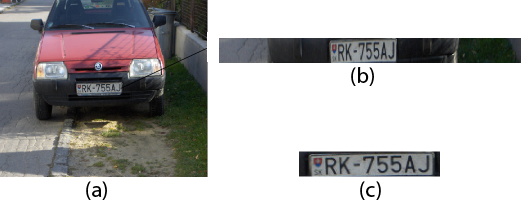
\includegraphics[scale=0.5, bb=0 0 598 212]{imagens/etapas2.PNG}
\end{center}
\caption{(a) Fotografia de um carro (b) \textit{Band} (c) \textit{Plate}.}
\label{fig:etapas2}
\end{figure}

    O m�todo de localiza��o do \textit{Band} inicia-se com um pr�-processamento na imagem do carro. Esse pr�-processamento consiste em aplicar um filtro de detec��o de arestas verticais (filtro de sobel - vertical) em uma imagem em escala de cinza. Esse processo � mostrado na Figura \ref{fig:etapa_3}.

\begin{figure}[!htb]
\centering
\begin{center}
    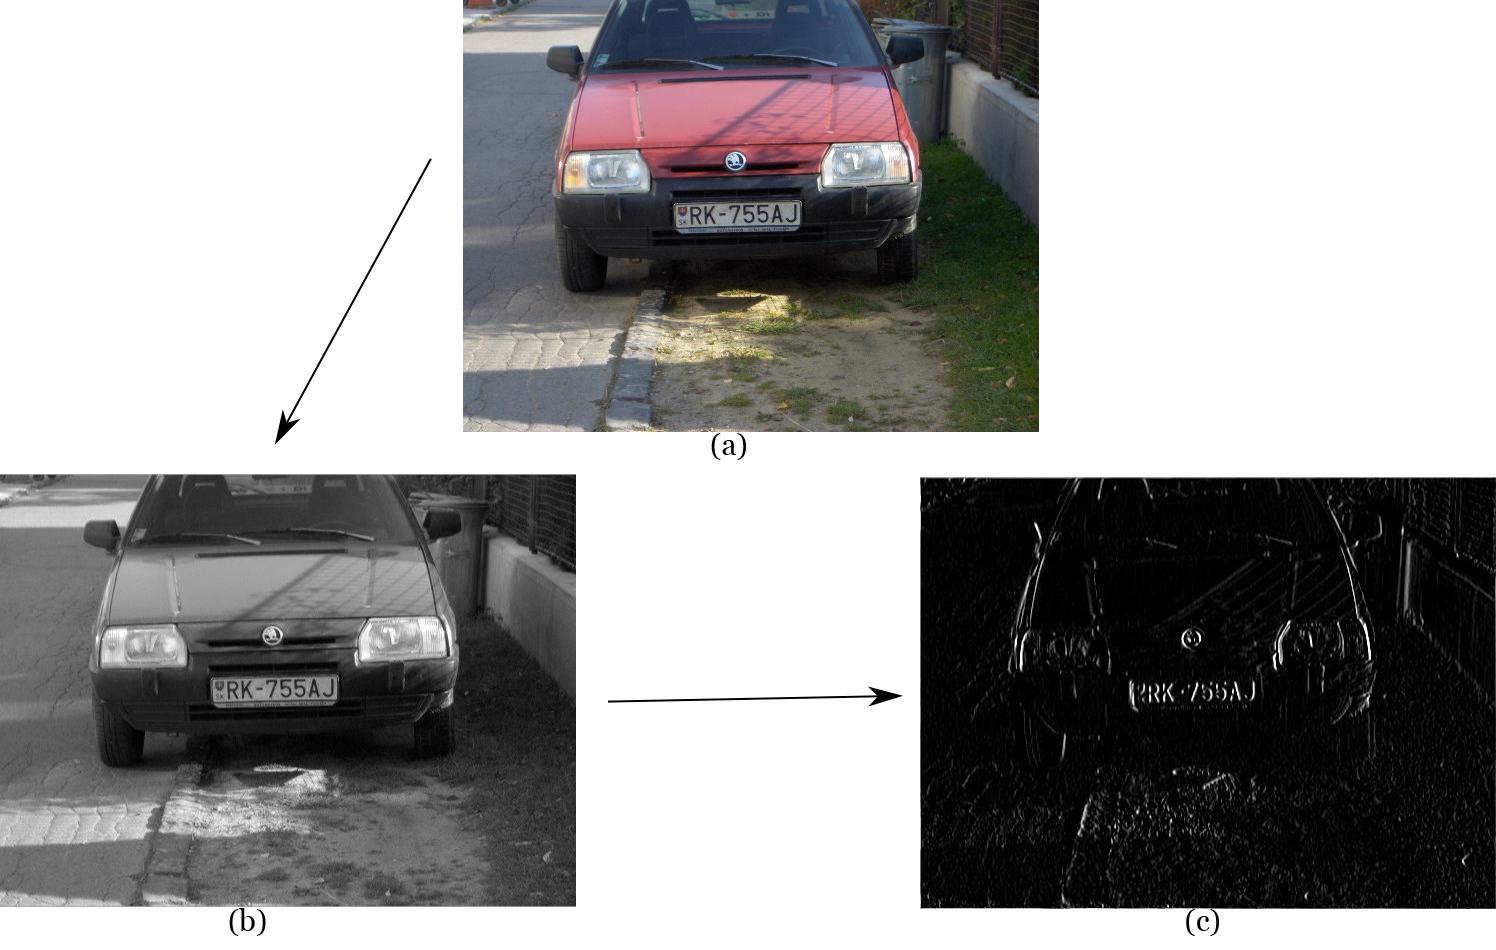
\includegraphics[scale=0.2, bb=0 0 1496 950]{imagens/etapa3.PNG}
\end{center}
\caption{(a) Fotografia de um carro (b) imagem convertida para escala de cinza (c) imagem filtrada por Sobel-Vertical.}
\label{fig:etapa_3}
\end{figure}   

    Ap�s o pr�-processamento aplica-se uma proje��o vertical. Essa proje��o consiste em somar a itensidade de cor dos pixels da imagem filtrada linha a linha. Matematicamente, pode-se definir a proje��o vertical como uma fun��o $pv: {0,...,h-1}\longrightarrow \mathbb{N}$ onde $pv(i)=\sum_{j=0}^{w-1} I(i,j)$ sendo $I:[0, w]\times[0, h]\longrightarrow{0,1,...,255}]$ a fun��o de intensidade de luz da imagem pr�-processada cuja largura � $w$ e altura � $h$. A Figura\ref{fig:etapa_4} mostra o exemplo de uma proje��o vertical de uma imagem de um carro.


\begin{figure}[!htb]
\centering
\begin{center}
    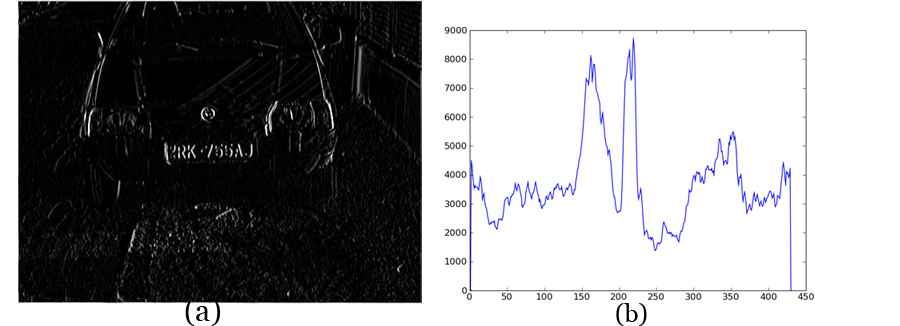
\includegraphics[scale=0.2, bb=0 0 1496 950]{imagens/etapa4.PNG}
\end{center}
\caption{(a) Imagem filtrada por Sobel-Vertical (b) Proje��o vertical.}
\label{fig:etapa_4}
\end{figure}   

    Analogamente, no processo de detec��o do \textit{plate} aplica-se um pr�-processamento, que difere-se do pr�-processamento do \textit{band} somente no fato que o filtro de detec��o de arestas usado � o filtro de sobel - horizontal. No resultado do pr�-processamento aplica-se uma proje��o horizontal. Essa proje��o � analoga a proje��o vertical. Soma-se, coluna a coluna, as intensidades de cor de cada pixel. Matematicamente a proje��o horizontal � dada pela fun��o $ph: {0,...,w-1}\longrightarrow \mathbb{N}$ onde $ph(j)=\sum_{i=0}^{h-1} I(i,j)$. A Figura \ref{fig:etapa_5} mostra o exemplo de uma proje��o horizontal de uma imagem de um \textit{band}.


\begin{figure}[!htb]
\centering
\begin{center}
    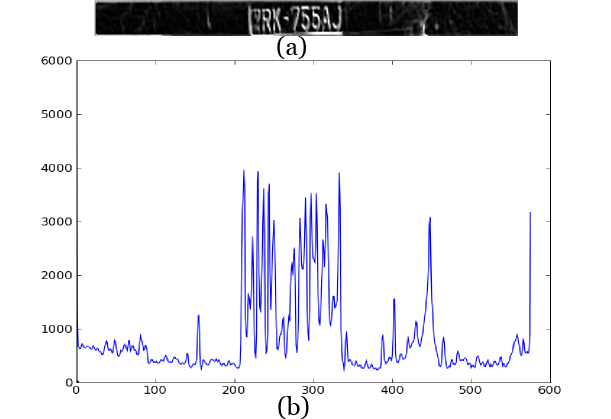
\includegraphics[scale=0.4, bb=0 0 611 419]{imagens/etapa5.PNG}
\end{center}
\caption{(a) Imagem do band pr�-processada (b) proje��o horizontal}
\label{fig:etapa_5}
\end{figure} 

    Normalmente o m�ximo global da proje��o vertical est� na regi�o que cont�m a placa. Isso se deve ao fato que em uma imagem de carro filtrada por Sobel-Vertical, normalmente, a regi�o da placa � a regi�o que cont�m mais arestas, e portanto essa � a regi�o que cont�m o m�ximo global da fun��o. Sendo essa uma fun��o discreta, o processo de dete��o de m�ximo global pode ser determinado por inspe��o, sem grandes custos computacionais. A esse valor de m�ximo global, denominaremos de \textit{pico}.

    Para definir o \textit{band} � necess�rio encontrar a linha inicial e a linha final da imagem do carro que o determinar�o. Para tal � necess�rio definir uma regi�o pr�ximo ao pico. A abordagem utilizada nesse projeto para definir essa regi�o divide-se em duas etapas. Na primeira, aplica-se uma suaviza��o na proje��o vertical. Para isso aplica-se um processo de convolu��o na imagem da fun��o proje��o. Essa convolu��o calcula a m�dia de valores em uma determinada vizinhan�a. Ap�s isso, na segunda etapa aplica-se uma fun��o \textit{threshold}, que consiste em, dado um valor $x$ que nesse caso � a m�dia dos valores da imagem da proje��o, para cada elemento da imagem da proje��o verifica se este � menor que $x$: caso seja, seu valor � zerado. Ap�s essa etapa, tem-se uma fun��o cuja imagem est� dividida em intervalos n�o nulos. Normalmente a placa est� no intervalo que cont�m o pico. Logo, basta extrair o �ndice inicial e o final que definem esse intervalo e consider�-los como as linhas inicial e final, respectivamente, usadas para o corte do \textit{band}. A Figura \ref{fig:etapa_6} mostra o processo de proje��o para determinar o \textit{band}.

\begin{figure}[!htb]
\centering
\begin{center}
    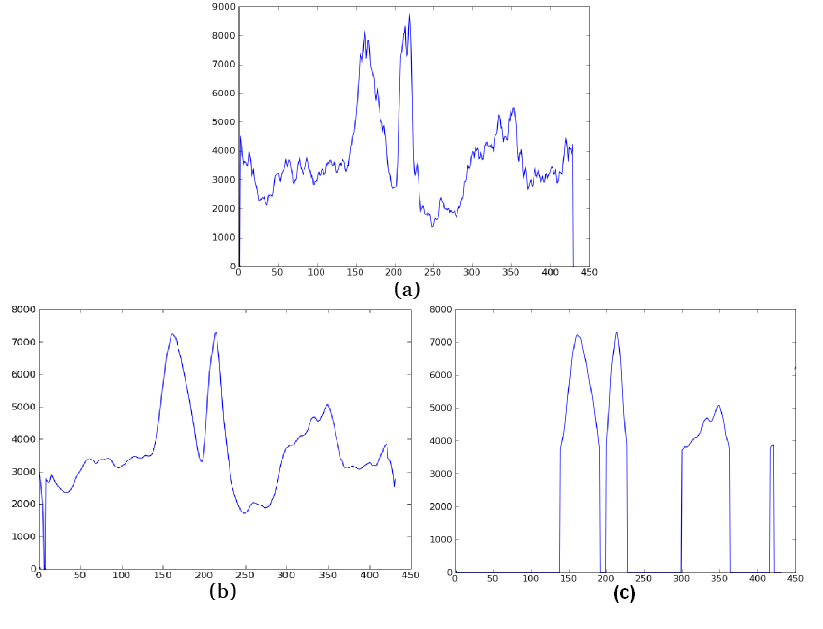
\includegraphics[scale=0.4, bb=0 0 823 629]{imagens/etapa6.PNG}
\end{center}
\caption{(a) Imagem original   (b) Proje��o vertical suavizada    (c) Aplica��o do \textit{Threshold}.}
\label{fig:etapa_6}
\end{figure} 

    O processo de detec��o do \textit{plate} � semelhante. Aplica-se a proje��o horizontal na imagem do \textit{band} pr�-processada, como dito anteriormente. Ap�s essa etapa, aplica-se as duas etapas de processamento na proje��o, assim como feito na proje��o vertical, o que resultar� em uma fun��o cuja imagem estar� dividida em intervalos n�o nulos. Normalmente a placa est� no intervalo de maior comprimento.

    Como dito ao longo do texto, esse processo n�o � determin�stico. Ele basea-se na alta probabilidade de acerto verificada empiricamente. Por�m, pode-se adotar algumas t�cnicas caso o \textit{band} adotado n�o seja o que contenha o pico. Isso pode acontecer quando alguma outra regi�o da imagem que contenha o carro contenha algum objeto com riqueza de detalhes, ou haja excesso de ru�dos concentrado em uma regi�o. Nessas possibilidades haver� regi�o de alta frequ�ncia, al�m da regi�o da placa. No caso do \textit{band}, pode-se ordenar os intervalos obtidos na etapa final ap�s a proje��o. Essa ordena��o basea-se em picos locais (picos nos intervalos). Ent�o os intervalos s�o organizados decrescentemente baseado nos picos locais. Vale destacar que o conjunto dos picos locais n�o � o conjunto de m�ximos locais, pois em um intervalo podem existir mais de um m�ximo local. Com essa ordena��o, continua-se o processo a partir do primeiro intervalo. Caso no fim do processo n�o encontre nenhuma placa, o processo com o \textit{band} � feito na segunda posi��o. Analogamente o \textit{plate} pode n�o estar no intervalo de maior comprimento. Dessa forma realiza-se uma ordena��o decrescente baseada no tamanho dos intervalos. Outra alternativa � utilizar algum m�todo para estimar a probabilidade de haver uma placa no \textit{band} e no \textit{plate}. Um m�todo que pode ser utilizado � a Transforada de Hough e verificar se existe um quadril�tero na regi�o determinada pelo \textit{band} ou \textit{plate}. Mais uma vez, esse � um m�todo probabil�stico. Por�m, vale destacar que a taxa de efici�ncia do PyANPR � satisfat�ria.

\section{Pr�-processamento da placa}

    Normalmente a imagem da placa cont�m ru�dos ou est� em uma baixa resolu��o. Esses fatores costumam baixar a taxa de acerto do reconhecimento dos caracteres (OCR). Para melhorar a qualidade da imagem, aumentando a taxa de acerto do reconhecimento de caracteres no PyANPR, adotou-se um processo dividido em tr�s etapas. Na primeira etapa, converte-se a imagem para escala de cinza. Na segunda extrai-se o ru�do atrav�s de um filtro de convolu��o cujo n�cleo basea-se na mediana. Por fim aplica-se um \textit{threshold} (se��o \ref{image:processing}). Um poss�vel valor do limiar � $128$, mas este pode ser alterado caso insira-se alguma outra etapa intermedi�ria. Uma etapa que pode ser utilizada � aplicar um filtro que realce arestas.

    Dessa forma, ap�s o pr�-processamento, obt�m-se uma imagem bin�ria da placa que servir� de entrada para a pr�xima etapa, a de reconhecimento de caracter.

 \section{OCR}
\label{sec:ocr}

   O \textit{toolkit} Horus disponibiliza diversos algoritmos para implementa��o de cada uma das etapas que constituem um sistema OCR (se��o \ref{sec:conceito_ocr}). Os algoritmos necess�rios para a constru��o das etapas de pr�-processamento e segmenta��o dos caracretes est�o dispon�veis no m�dulo de processamento de imagens do Horus, alguns desses algoritmos s�o: detec��o de arestas, binariza��o, suaviza��o, remo��o de ru�dos, proje��es, entre diversos outros algoritmos.

Ap�s a segmenta��o dos caracteres, extrai-se um vetor n�merico (vetor de caracter�sticas) de cada um desses. Tal vetor � utilizado como padr�o de entrada para uma rede neural no processo de reconhecimento. 
O processo de extra��o de caracter�sticas � uma das etapas mais importantes de um sistema OCR, a qualidade dessa etapa influencia no resultado de todo o sistema. Portanto, a escolha de quais caracter�sticas ser�o utilizadas como padr�o de entrada no processo de reconhecimento � extremamente importante. A constru��o do vetor de caracter�sticas pode ser feito utilizando os diversos algoritmos implementados no m�dulo de extra��o de caracter�sticas do Horus (se��o \ref{sec:features}) podem ser: histograma de arestas por regi�es, termina��o de linha, \textit{loops}, entre outros. Por �ltimo, � realizado a etapa de reconhecimento do vetor de caracter�sticas, que finalmente dever� apontar o caractere correto. Uma abordagem usual para a contru��o da etapa de reconhecimento consiste na utiliza��o de redes neurais artificiais (se��o \ref{sec:rna}). O Horus disponibiliza algoritmos para cria��o e utiliza��o de redes neurais atrav�s de uma API \textit{Open Souce} chamada \textit{Fast Artificial Neural Network}(FANN). 

 Atualmente, o \textit{toolkit} Horus n�o possui um sistema OCR pr�prio, essa funcionalidade ser� implementada em um trabalho futuro. Por�m, esse \textit{toolkit} disponibiliza funcionalidades de um sistema OCR atrav�s da utiliza��o de um OCR \textit{Open Source} chamado Tesseract.  
   
   
\section{Aplica��o Web}
    Durante o desenvolvimento deste trabalho, mais especificamente do sistema PyANPR, foi desenvolvido um sistema web cujo objetivo �: atrav�s do \textit{upload} de uma imagem de um carro, o sistema realizar� o ANPR nessa imagem e retornar� todas as informa��es da placa contidas em seu banco de dados. 
    Esse sistema foi constru�do utilizando um \textit{framework} \textit{web} de alt�ssimo n�vel chamado Django. Esse \textit{framework} � escrito na linguagem de programa��o Python e � baseado no padr�o arquitetural \textit{Model View and Controller}(MVC) \cite{Fowler2003}. 

%%%%%%%%%%%%%%%%%%%%%%%%%%%%%%%%%%%%%
%%  O Tool Kit Horus
%%%%%%%%%%%%%%%%%%%%%%%%%%%%%%%%%%%%%


\chapter{O Toolkit Horus}
\label{cap:o_toolkit_horus}

O Horus � um toolkit, ou seja, uma cole��o de ferramentas (nesse caso m�dulos) que servem para gerenciar agentes inteligentes, escrito em Python. Duas partes est�o sendo desenvovdidas a princ�pio: M�dulo de Vis�o e M�dulo de Mapeamento.

No m�dulo de vis�o est�o os mais variados algoritmos de vis�o computacional e no m�dulo de mapeamento trata-se do problema de mapear ambientes a partir de dispositivos de leitura do ambiente e de efetuadores.
\section{Objetivo}

O objetivo do toolkit � prover ferramentas necess�rias para produ��o de agentes inteligentes. 

\section{Arquitetura}

Demonstrar a arquitetura utilizada.

\section{M�dulos do Horus}

Principais funcionalidades de cada um dos m�dulos, de forma mais explicada. .
\
\begin{itemize}
\item Core do Horus: Cont�m m�dulos que ser�o utilizados como suporte para os m�dulos principais. Sendo assim n�o necessitam ser utilizados diretamente pelo usu�rio.
\item Modulo de Vis�o: Tem por objetivo tratar as principais t�cnicas de vis�o computacional de um agente inteligente.
\item Modulo de Mapeamento: O m�dulo de mapeamento � respons�vel por gerenciar os tipos de mapeamento bem como os dispositivos utilizados para mapear e navegar no ambiente.
\end{itemize}

\subsection{Core do Horus}
As fun��es e m�todos presentes no Core do Horus est�o dispostas como segue:

\subsubsection{O m�dulo "math\textunderscore module"}
Este m�dulo possui fun��es matem�ticas usadas pelo Horus. Ele est� subdividido em algumas categorias dentre elas, fun��es trigonom�tricas e regress�o linear.

As fun��es trigonom�tricas s�o:
\begin{itemize}
\item \textbf{getXCateto(self, hypotenuse, angle)} - respons�vel por encontrar a coordenada X em um plano cartesiano tendo como par�metros a dist�ncia (hipotenusa) at� o ponto e o �ngulo de rota��o atingido para observar aquele ponto.

\item \textbf{getYCateto(self, hypotenuse, angle)} - respons�vel por encontrar a coordenada Y em um plano cartesiano tendo como par�metros a dist�ncia (hipotenusa) at� o ponto e o �ngulo de rota��o atingido para observar aquele ponto.

\item \textbf{isPointInCircle(self,  center\textunderscore tuple,  point\textunderscore tuple,  radius)} - respons�vel por definir se um ponto (X, Y) qualquer est� ou n�o contido em um c�rculo, dado o centro deste e o raio.
\end{itemize}

A fun��o de regress�o linear � respons�vel por fazer uma identifica��o de uma condicional de uma vari�vel y, tendo dados de v�rios x.

\textbf{COMPLETE WALLACE}


\subsubsection{O m�dulo "processingimage"}
Nesse m�dulo est� definido o processo de tratamento de imagem.



\subsection{M�dulo de Vis�o}

\subsection{M�dulo de Mapeamento}

O m�dulo respons�vel pela intelig�ncia do agente, no que diz respeito � localiza��o, movimenta��o, mapeamento e navega��o. 
\begin{itemize}
\item Localiza��o: Entende-se por localiza��o a capacidade do agente localizar-se em um ambiente. 
\item Movimenta��o: � a capacidade de locomo��o em um ambiente.
\item Mapeamento: � o modo como o agente localiza marcos para identificar a forma do ambiente.
\item Navega��o: O agente se move pelo ambiente mapeado visando um objetivo, com tarefas como otimiza��o de rotas.

\end{itemize}

%%%%%%%%%%%%%%%%%%%%%%%%%%%%%%%%%%%%%
%%  Mapeamento
%%%%%%%%%%%%%%%%%%%%%%%%%%%%%%%%%%%%%


\chapter{Mapeamento}
\label{cap:mapeamento}

%%%%%%%%%%%%%%%%%%%%%%%%%%%%%%%%%%%%%
%%   Aplica��o do ambiente virtual com um rob� aut�nomo
%%%%%%%%%%%%%%%%%%%%%%%%%%%%%%%%%%%%%


\chapter{Aplica��o do ambiente virtual com um rob� aut�nomo}
\label{cap:aplicacao_autonomo}
A fim de produzir uma prova de conceito, foi implementada uma aplica��o onde foi poss�vel demonstrar a efici�ncia do algoritmo de mapeamento. Foi produzido um simulador com gravidade, colis�o, rederiza��o de texturas, objetos e atores (o agente nesse caso) e, tendo esse simulador como base, foi criada a aplica��o que tem um agente utilizando-se do Toolkit H�rus para mapeamento e navega��o dentro do ambiente simulado.
\section{Simulador}
O simulador desenvolvido foi tratado como uma aplica��o a parte, pois n�o estava inclu�do no escopo do projeto, por�m tendo em vista a necessidade de um simulador customizado para a realidade de um agente m�vel (e na linguagem selecionada) o simulador foi incluido ao projeto. 

\subsection{Requisitos para o ambiente virtual}
Foram utilizados alguns softwares para que fosse poss�vel a cria��o e renderiza��o do ambiente. Esses softwares foram: Blender e Panda3d.
Como uma das linguagens utilizadas foi Python, buscou-se ferramentas que fossem compat�veis (na verdade ambas s�o em Python) com as linguagens utilizadas.

O Blender � um produto da Blender Fundation, que � open source e desenvolvido em Python para modelagem de objetos 3D que est� dispon�vel para v�rios sistemas operacionais sobre a licen�a GNU (General Public License).

O Panda3D � um produto da equipe de desenvolvimento da Walt Disney para renderiza��o de jogos e ambientes virtuais em terceira dimens�o. Est�o sobre licen�a da BSD License (com algumas modifica��es para adequa��o a realidade do projeto).

\subsection{Ambiente}
O ambiente em que o rob� foi testado consiste em uma �rea que simula um galp�o com 5 c�modos onde o agente inicia sua movimenta��o no c�modo 1 e pode alcan�ar qualquer ponto do ambiente a partir de sua posi��o inicial. O ambiente que foi desenvolvido tem como objetivo emular, em menor escala, um ambiente real.

O ambiente que foi utilizado foi modelado em Blender, tal ferramenta proporcionou os recursos de modelagem UV, texturiza��o, determina��o de medidas precisas, entre outros, assim como uma legibilidade de f�cil assimila��o tendo em vista que o Toolkit foi desenvolvido em Python e a ferramenta utiliza a mesma linguagem para produzir os modelos.

\begin{figure}[htb]
\centering
\includegraphics[scale=0.5,bb=0 0 390 550]{imagens/fotos/galpao.png}
\caption{O ambiente utilizado para a prova de conceito.}
\label{fig:ambiente}
\end{figure}

Na figura \ref{fig:ambiente}, que demonstra o ambiente que foi utilizado, pode-se ter uma vis�o em perspectiva do ambiente modelado.

%%%%%%%%%%%%%%%%%%%%%%%%%%%%%%%%%%%%%
%%   Resultados
%%%%%%%%%%%%%%%%%%%%%%%%%%%%%%%%%%%%%


\chapter{Resultados obtidos}
\label{cap:aplicacao_autonomo}


%%
%%Inluir todos os capitulos aqui
%%\include{file}
%%

%%%%%%%%%%%%%%%%%%%%%%%%%%%%%%%%%%%%%
%%   CONCLUS�ES E TRABALHOS FUTUROS
%%%%%%%%%%%%%%%%%%%%%%%%%%%%%%%%%%%%%


\chapter{Conclus�es e Trabalhos Futuros}
\label{cap:conclusao}

H� muito que melhorar para garantir que o processo de mapeamento seja mais produtivo.

Como trabalhos futuros iremos em primeiro momento concluir o ransac, m�todo respons�vel por encontrar landmarks a partir de pontos extra�dos com leitura de lasers. Com isso, o agente ser� capaz de identificar paredes e poder� us�-las para a sua navega��o e mapeamento.

Apesar de o m�todo ransac estar pronto e fazer parte do nosso m�dulo SLAM, ele ainda n�o est� em uso, pois n�o foi necess�rio no ambiente-tarefa das aplica��es. Contudo, testes individuais executados no m�todo indicam um bom funcionamento com taxas de erros muito baixa. Entretanto na aplica��o o numero de \textit{landmarks} encontrados esta abaixo do esperado. Os ajustes no ransac ser�o o de desconsiderar as leituras dos lasers das pontas, por possu�rem uma discrep�ncia em rela��o a outras leitoras e gerarem erro no RANSAC, excluir os pontos com o valor considerado infinito na aplica��o e fazer o calculo do intervalo de confian�a da linha encontrada.

Com o RANSAC pronto iniciaremos o m�dulo que criar� um grafo completo a partir dos marcos encontrados. Com os landmarks � poss�vel fazer a poda do grafo e usar esse grafo para buscar o melhor caminho com algoritmo gen�tico.
No atual ambiente tarefa n�o foram considerados os erros dos sensores. No entanto, com a adi��o desses erros, m�dulos de tratamento de incerteza utilizando L�gica \textit{Fuzzy} e Filtro de \textit{Kalman} passar�o a entregar o Horus.

\end{spacing}

%Include da bibliografia
\begin{spacing}{1.0}
%%%%%%%%%%%%%%%%%%%%%%%%%%%%%%%%%%%%%
%%   Bibliografia
%%%%%%%%%%%%%%%%%%%%%%%%%%%%%%%%%%%%%
\bibliographystyle{abnt-alf}
\bibliography{biblio}


\end{spacing}

%Include do ap�ndice
\begin{spacing}{1.5}
%%%%%%%%%%%%%%%%%%%%%%%%%%%%%%%%%%%%%
%%   AP�NDICE
%%%%%%%%%%%%%%%%%%%%%%%%%%%%%%%%%%%%%


\appendix
\addcontentsline{toc}{chapter}{Ap�ndices}

\chapter[Depend�ncias do Tool kit]{Depend�ncias do Tool kit}

M�dulos Python para o funcionamento completo do toolkit:
\begin{itemize}

\item FANN [http://leenissen.dk/]

\item MATPLOTLIB [http://matplotlib.sourceforge.neT/]

\item NUMERICS [http://numpy.scipy.org/]

\item PIL [http://www.pythonware.com/products/pil/]

\item SWIG [HTTP://www.swig.org/]

\item TESSERACT [http://code.google.com/p/tesseract-ocr/]

\end{itemize}

\chapter[Siglas]{Siglas}

\begin{itemize}
\item SLAM - Simultaneos Location and Mapping
\item IA - Intelig�ncia Artificial
\item NASA - National Aeronautics and Space Administration
\item MEFA - Mm�quina de Estados Finitos Ampliadas
\item RANSAC - Random Sampling Consensus
\item GNU - General Public License
\item UV - Refere-se a latitude e longitude.

\end{itemize}

\end{spacing}

\end{document}
